%--------------------------------------
% Master's Thesis Title Page 
% LaTeX Template
% Version 1.0 (23/05/14)
% Thanks to Magnus Marthinsen, this thesis and template is made available for Master studentes at HVL Joint SE program (01.03.2021)
%---------------------------------------

%----------------------------------------------------------------------------------------
%	PACKAGES AND OTHER DOCUMENT CONFIGURATIONS
%----------------------------------------------------------------------------------------
\documentclass[a4paper]{report} 
\usepackage{graphicx} % Required for box manipulation
\usepackage{helvet}
\usepackage{subfig}
\usepackage[utf8]{inputenc}
%\usepackage{natbib}
\usepackage[USenglish]{babel}
\usepackage[useregional]{datetime2}
\usepackage{pgfgantt}
\usepackage{listings}
\usepackage{wrapfig}
\usepackage{setspace}
\usepackage{parskip} % Used to create spaces between paragraphs
\usepackage{dirtytalk} % quotes by talk
\usepackage[hidelinks]{hyperref}
\usepackage[acronym, toc]{glossaries}  % Used to add a wordlist/glossaries
\usepackage{amsfonts} 
\usepackage{color, colortbl}
\usepackage{booktabs}
\usepackage{float}
\restylefloat{table}
\usepackage{csquotes}
\usepackage{amsmath,amssymb} 
\usepackage{ulem}
\usepackage{longtable}
\usepackage{array}
\usepackage[left=3cm, right=3cm, top=3cm, bottom=3cm]{geometry}
\renewcommand{\arraystretch}{1.5}
%BIB by Adrian
\usepackage[backend=biber,style=numeric, urldate=long]{biblatex}
% See the references.bib file. Most Bibtex bibliographies in Computer Science can be found from dblp.org 
\addbibresource{references.bib}


\newread\tmp

\newcommand{\quickcharcount}[1]{%
  \immediate\write18{texcount -1 -sum -merge -char #1.tex > #1-chars.sum}%
  \openin\tmp=#1-chars.sum%
  \read\tmp to \thechar%
  \closein\tmp%
}

\newcommand{\quickwordcount}[1]{%
  \immediate\write18{texcount -1 -sum -merge #1.tex > #1-words.sum}%
  \openin\tmp=#1-words.sum%
  \read\tmp to \theword%
  \closein\tmp%
}

% Glossary/wordlist
\makeglossaries
%\newglossaryentry{local_maximum}
%{
%    name={local maximum},
%    description={When performing optimizations there might be several viable solutions. Some methods might find the closest viable solution from the starting point (local maximum), even though there might exist a better solution in the environment. The best solution in the environment is a global maximum}
%}

\newacronym{MDSE}{MDSE}{Model Driven Software Engineering}
\newacronym{SE}{SE}{Software Engineering}
\newacronym{DEPA}{DEPA}{Danish Environmental Protection Agency}
\newacronym{QA}{QA}{Quality Attributes}
\newacronym{QAS}{QAS}{Quality Attribute Scenarios}
\newacronym{MVP}{MVP}{minimum viable product}
\newacronym{AI}{AI}{Artificial Intelligence}
\newacronym{EO}{EO}{Earth Observation}
\newacronym{JWT}{JWT}{JSON Web Token}
\newacronym{GeoTIFF}{GeoTIFF}{Geographic Tagged Image File Format}
\newacronym{OOP}{OOP}{Object-oriented programming}
\newacronym{AWS}{AWS}{Amazon Web Service}
\newacronym{hdfs}{HDFS}{Hadoop Distributed File System}
\newacronym{GB}{GB}{gigabyte}
\newacronym{GIS}{GIS}{Geographic Information System}
\newacronym{wkt}{WKT}{Well-known text}
\newacronym{BBox}{BBox}{bounding box}
\newacronym{GIL}{GIL}{Global Interpreter Lock}

\begin{document}

%
% COLORS USED THROUGH THE REPORT
%
\definecolor{kb_red}{RGB}{96,2,4}
\definecolor{light_gray}{RGB}{160,160,160}
\definecolor{med_gray}{RGB}{96,94,94}
\definecolor{black}{RGB}{0,0,0}
\definecolor{white}{RGB}{155,155,155}
\definecolor{light_green}{RGB}{208,240,192}
\definecolor{light_red}{RGB}{255,204,203}

% CODE STYLE
\definecolor{javared}{rgb}{0.6,0,0} % for strings
\definecolor{javagreen}{rgb}{0.25,0.5,0.35} % comments
\definecolor{javapurple}{rgb}{0.5,0,0.35} % keywords
\definecolor{javadocblue}{rgb}{0.25,0.35,0.75} % javadoc
 
\makeatletter
\lst@Key{matchrangestart}{f}{\lstKV@SetIf{#1}\lst@ifmatchrangestart}
\def\lst@SkipToFirst{%
    \lst@ifmatchrangestart\c@lstnumber=\numexpr-1+\lst@firstline\fi
    \ifnum \lst@lineno<\lst@firstline
        \def\lst@next{\lst@BeginDropInput\lst@Pmode
        \lst@Let{13}\lst@MSkipToFirst
        \lst@Let{10}\lst@MSkipToFirst}%
        \expandafter\lst@next
    \else
        \expandafter\lst@BOLGobble
    \fi}
\makeatother
 
\lstset{language=Java,
basicstyle=\footnotesize,
keywordstyle=\color{javapurple}\bfseries,
stringstyle=\color{javared},
commentstyle=\color{javagreen},
morecomment=[s][\color{javadocblue}]{/**}{*/},
numbers=left,
captionpos=b,
frame=single,
breakatwhitespace=false,
breaklines=true,
numberstyle=\tiny\color{black},
stepnumber=1,
numbersep=10pt,
tabsize=2,
showspaces=false,
showstringspaces=false,
matchrangestart=t}

%Title page
\pagenumbering{roman}
\begin{titlepage}

    \begin{center}
        \vspace*{1cm} % Adjust this value to position content vertically

        % Title
        {\Huge \textbf{Satellite-Based Detection of}}\\[2mm]
        {\Huge \textbf{Pesticide Overuse}}\\[3cm] % Main title, adjust text as needed

        % Authors' names and IDs
        {\Large Oskar Thomsen \hspace{16mm} 23123}\\
        {\large \hspace{4mm} \textit{achri20@student.sdu.dk}}\\[5mm]
        {\Large Anton Christensen \hspace{10mm} 23123}\\
        {\large \hspace{4mm} \textit{achri20@student.sdu.dk}}\\[12mm]
        


        % Degree information
        {\large \textit{Master’s Thesis in Software Engineering}} \\[0.8cm]

        % Advisor information
        \textit{Advisor: Aslak Johansen} \\
        \hspace{6mm}\textit{achri20@student.sdu.dk} \\[2.5cm]
        

        % Date
        {\large June 2025} \\[6cm]

        % SDU Logo at the bottom
        
\includegraphics[width=0.3\linewidth]{images/logos/SDU_BLACK_RGB_1.png} \\[1cm] % Adjust logo size and spacing if needed

        % University and department information
        \textit{The Maersk Mc-Kinney Moeller Institute} \\
        \textit{University of Southern Denmark} \\
    \end{center}

\end{titlepage}

\pagebreak

\section*{Abstract}
\acrlong{MDSE} is a ...

\section*{Acknowledgements}
First and foremost, I would like to thank ...

\quickwordcount{main}
\quickcharcount{main}

There are \thechar characters and approximately \theword spaces.
That makes approximately \the\numexpr\theword+\thechar\relax\ characters total. out of 144000

\pagebreak
\tableofcontents
\listoffigures
\listoftables

\printglossary[nonumberlist]
\printglossary[type=\acronymtype, nonumberlist]
\newpage

\pagenumbering{arabic}
\chapter{Introduction} \label{Intoduction}
This thesis looks at the development of a software system for the Danish Environmental Protection Agency, with the purpose of helping them to uphold the regulations put in place regarding pre-harvest crop desiccant use. It will cover the necessary agricultural knowledge regarding Danish potato production and crop desiccation methods, as well as exploring how satellite imagery can be used to monitor crop health over time, and by extension, whether crop desiccant usage can be monitored in relation to the desiccation time of crops. The remaining sections in the introduction will provide further insight into the case presented by the Danish Environmental Protection Agency, the problem the authors are attempting to solve, how the case was approached and important terminology. A reading guide is presented at the end to help navigate the thesis report.

\section{Collaboration with the Danish Environmental Protection Agency}
The \acrfull{DEPA} (da: Miljøstyrelsen)(DEPA) is a government agency that deals with a variety of tasks related to Danish business, industry, agriculture, and consulting companies and business organizations, to further Danish interests while ensuring environmental progress\cite{MiljøstyrelsenOpgaver}. One such task is upholding the regulations put in place in regards to pre-harvest crop desiccant usage in the agricultural sector, to prevent pollution of nearby ecosystems and the ground water. The \acrshort{DEPA} contacted The University of Southern Denmark (SDU) through a representative with a project case, that could help uphold the pre-harvest crop desiccant regulations. Thus, this representative was the primary contact person from the DEPA for the authors throughout the project.


\section{Context}
The following section is an introduction into the case presented by the DEPA representative and gives further context into problem they are facing and how it could potentially be solved using satellite imagery. Additionally, the case presentation can be found in appendix(INDSÆTPP).

Pre-harvest crop desiccants are commonly used for wilting crops on fields. Ensuring that all plants are dead and wilted will significantly diminish the bacteria and parasites that are left to carry over to the next year, thus improving the fundamental conditions for future harvests\cite{europaAgriculturePesticidesplant}. But pesticides have been shown to seep into the ground water, which poses significant health implications\cite{pesticiderGrundvand} and to be damaging to nearby wildlife ecosystems\cite{Middeldatabasen}. In order to restrict the rate of this pollution, regulations made by the DEPA have been put in place for how much and how often pesticides are allowed to be sprayed. To uphold these regulations, mandated annual inspections are performed. But considering that 60.4\% of Denmark's landscape is utilised for the agricultural sector\cite{Lindsgaard2017-em}, that the number of mandated annual inspections are below 1000 a year (746 inspections in 2019)\cite{MiljoeOgFoedevareministeriet}, and that the inspections are random rather than being informed by some observations, the chances of getting caught for an overuse of pesticides are slim. 

A map of the NDVI index can be produced from data collected by the Sentinel 1 through 6 satellites from the Copernicus Expansion Missions\cite{noauthor_undated-bb}. Normalized Difference Vegetation Index (NDVI) is a common index of vegetation health used in remote sensing\cite{GISGeography2017-cr}. Healthy vegetation reflects more near-infrared light and absorbs more visible red light, resulting in a higher NDVI value. In contrast, stressed vegetation absorbs more near-infrared light and reflects more red light, leading to a lower NDVI value. The scale of NDVI goes from -1 to 1, where a 1 would be a healthy plant and 0 would indicate no healthy vegetation or an urbanised area. A negative NDVI index would indicate an ocean\cite{GISGeography2017-cr}. With this information one should be able to deduce whether there are stressed or wilting crops on fields and how quickly the wilting happens, if monitored over time. 

A quicker than usual wilting process may be an indication of an overuse of pesticides, which is in violation of the regulations, and such an observation might warrant an inspection. By inspecting those crops that are more likely to have been wilted using pesticides, the hit rate of inspections should rise. The number of farmers that will get fined for this overuse will produce additional funding that can lead to a more balanced risk scenario for the farmers, resulting in less pesticide use and thus less pollution of the ground water and nearby wildlife ecosystems.


\section{Problem}
What would it take to implement a system for finding inspection site candidates, and how efficient would it be in finding overuse of pre-harvest crop desiccants?
\vspace{1em}

\noindent In particular,
\begin{enumerate}
    \item \textbf{Model:} How can satellite data be analysed to define a statistical model of crop wilting where NDVI is defined as a function over time? Such a model should be parameterised over geography and type of crop.
    \item \textbf{Validation:} Can such a model be used to detect crop desiccation rates that fall outside the model and detect pre-harvest crop desiccant use?
    \item \textbf{Scale:} How can such a model be implemented efficiently, for all crop fields in Denmark?
\end{enumerate}

\section{Approach}
Historical observations of normal crop desiccation timelines will be used to train and build a models of a single crop type commonly produced in Denmark.
One model will be produced for normal wilting and another for desiccant accelerated wilting. Open-access Sentinel data will be used for this, and ground truth from DEPA will be used to differentiate between normal and accelerated wilting.
This will allow the observed wilting process of any field to be compared to the normal model and the accelerated model, and based of such comparisons a likelihood of crop desiccant use can be determined.
Cross-validation using the ground truth from DEPA will be performed to evaluate to which degree the model-pair is capable of differentiating between normal and accelerated wilting. Once such differentiation is possible, finding outliers from both models, which could also be an indication of pesticide overuse, is possible.

Starting off, the model will be trained to detect accelerated wilting in potato plants, by request of the DEPA. Then, to scale the model, other crop types will be chosen for training and validation. The whole model will then be deployed on a cloud service with big data techniques to ensure that the DEPA can scale and launch the monitoring service for different crop types and find outlier from the model, prompting a site inspection.


\section{Terminology}
Vi udpensler allerede NDVI ret godt i context afsnittet, men vil gerne lige snakke om hvilke andre terminologier vi evt skal have fat i. Evt sådan noget "hvad mener vi, når vi siger "crop wilting" eller "model for crop wilting over time" eller whatever"

\section{Reading Guide}
Skrives senere
\chapter{Process}\label{Process}
\textcolor{red}{some small text about what process is going to be about }

\section{Project Timeline}

\textbf{Initial TimeLine} 
\textcolor{red}{Talk about the first timeline created and a link to appendix where it is }

\textbf{Actual Timeline}
\textcolor{red}{Talk about the timeline that actulley happened}

\textbf{The difference}
\textcolor{red}{Talk about why and what the differences are is it just lazyness or where there actuel problems and where we to optimistik}

\textcolor{red}{the actuel timeline figure}
\section{Development process}
\textcolor{red}{So this should be about that we are going to be working in an iterative work style where there is a goal for each week and we end the week wiht a pick up }
\chapter{\textbf{Domain} Analysis} \label{Analysis}
This section will cover an analysis of the case presented by the \acrshort{DEPA} in section 3.1 and what challenges it presents. From then it will delve into necessary knowledge required to develop a solution for the case, starting with some ground truths regarding potato agriculture in Denmark in section 3.2. Monitoring of potato crops will be performed using the Copernicus Satellite API, which is described in section 3.3 along with the satellite capabilities. Finally, the remote sensing data from the satellites can be used to calculate vegetation indices, which are explored in section 3.4 and the differences between the vegetation indices.

\section{Analysis of the stakeholder presentation} \label{Analysis of the stakeholder presentation}
During the case presentation with the representative from the \acrshort{DEPA}, it was clear that they wanted a more optimal way of checking inspection site candidates for potential pesticide overuse checks. Currently they employ a limited number of random agricultural soil samples on different sites each year\cite{MiljoeOgFoedevareministeriet}, which potentially results in pesticide overuse going unnoticed. To combat this, the case presented a solution to use satellite image data and using NDVI index over time, to see if there is an abnormal drop in NDVI index, which could be an indicator for pesticide overuse.
This presents some additional challenges, as different crop types are sprayed with pesticides for various reasons and at varying times during the year, depending on the type of crop. In accordance to this, the \acrshort{DEPA} had a specific use case regarding seed potatoes and the use of the pesticide Reglone\cite{reglone / case PP} that is used for pre-harvest crop desiccation. The proposed solution is to look for a drop in the NDVI index from the satellite imagery from seed potato fields, which would indicate that pesticide use for pre-harvest crop desiccation has been employed, and then to search for fields where the NDVI index drops off faster than the norm, which could be an indicator of overuse.

To be able to perform this task, the following section will delve into potato farming standards and practices and necessary knowledge.

\section{Potato knowledge} \label{Potato knowledge}
There are several potato types that being sown and harvested in Denmark. Most commonly, table/eating potatoes for consumption (da: spisekartofler), seed potatoes for planting (da: læggekartofler) and starch potatoes grown for potato starch production (da: melkartofler).
This is an umbrella term that encapsulates a variety of different potatoes in each potato type. Some varieties of potatoes have earlier harvests and/or could require different growth environments, in terms of soil nutrients and moisture. 

\subsection{Growth period} \label{Growth Period}
Potatoes are planted in late March and throughout April where the soil is around 8 degrees Celsius and the soil has the correct moisture levels\cite{LandbrugogFødevarer}. Before planting the field has been ploughed and is divided into trenches with approximately 75 cm between each trench, leaving space for machinery to drive by, without damaging the potatoes. In the trenches the potatoes are planted with proximately 20-33 cm distance between each other and covered with 6-8 cm layer of dirt\cite{LandbrugogFødevarer}. Once planted the potato takes anywhere from 2-6 weeks to germinate, depending of soil temperature, moisture and pH levels\cite{vegtotable_potato_germination}.

Harvesting season varies depending on the type and potato variety. Some table potatoes are harvested in June throughout July, while others are being harvested throughout August till October, which affects both size and taste of the table potatoes. Seed potatoes are harvested in the later months, August throughout October, to ensure they are large enough and carry enough nutrients for a healthy harvest the following year\cite{PPOplæg}.

\subsection{Pests and diseases}\label{Pests and diseas}
During the early growth period, before the potato seeds start sprouting out of the ground the field is bare. This enables weeds to get enough light to start growing, until the potato sprouts are tall enough to cover the ground, closing light off from the weeds which prevents their growth. Combating weeds in the early growth period can be done chemically using pesticides or mechanically using machinery\cite{LandbrugogFødevarer}.

Insect pests can attack the potatoes from both the sprouts and the roots, which negatively effects the yield and the quality of the potatoes. Whether pesticides are used to combat these pests is dependent on the severity of each case, usually determined by the amount of insects per potato plant\cite{InsectPests}.

Additionally, the potatoes can be inflicted by plant diseases, most notably potato blight. Potato blight is a fungus that, if goes untreated, causes the potato to rot and become inedible. To combat potato blight, the farmer can employ practices such as only planting healthy potatoes, hill the potatoes in relation to sprout growth to lessen the chance that the potato tuber gets infected and spray with an agent that prevents the fungus growth regularly\cite{PotatoBlight}. 

\subsection{Pre-harvest desiccation agents} \label{Pre-harvest desiccation agents}
There is a variety of pesticides. Herbicides, that focus on combating weeds or other plant matter, Insecticides, for killing insect pests and fungicides, to prevent fungal based plant sickness\cite{pesticiderUmbrellaterm}. And while a variety of different pesticides are used throughout the year to combat pests and diseases, the focus point presented by the case is the use of herbicides, specifically pre-harvest crop desiccation agents for seed potatoes in August throughout October.
The \acrshort{DEPA} stated that the monitoring of the pre-harvest desiccation agent Reglone was the focus point of the case\cite{oplægPP}. 

Reglone is a pre-harvest crop desiccation agent used on potatoes for storage (E.g.. seed potatoes). Reglone is a contact agent that is sprayed on the green sprouts growing out of the potato tuber and with the help of sunlight it creates hydrogen peroxide, wilting the plant. The agent is highly effective and dessication can be seen within 3-10 days. A maximum of two dosages is allowed and last dosage no longer than seven days prior to harvest\cite{Middeldatabasen}.

During the interview with the agricultural school, the two teachers interviewed mentioned that Reglone was hardly ever used due to regulations and most potato farmed had resorted to using milder pre-harvest desiccation agent, Mizuki\cite{interview}. Mizuki is also a contact agent and only used for potatoes for storage (E.g. seed potatoes). While the effect of Mizuki is not as immediately present as Reglone, it is highly effective and desiccates the plant after 14-21 days. Two dosages are allowed with a five day gap and the last application can be no longer than seven days prior to harvest\cite{Middeldatabasen}.

\subsection{Dangers of pre-harvest desiccation agents} \label{Dangers of pre-harvest desiccation agents}
Both Reglone and Mizuki are corrosive liquids and needs to be handled using gloves, masks and eye protection. Coming in contact with the agents causes skin irritation and needs to be washed off immediately. Breathing in the mist from the agents can cause irritation in the airways and in severe cases cause irreparable lung damage or even death\cite{Middeldatabasen}.
Besides being harmful to humans, regulations state that the agents must not be applied closer than 30 meters from aquatic environments (lakes, rivers, etc.) and 20 meters from § 3-areas, which includes wild vegetation\cite{Paragraf3}\cite{Middeldatabasen}. This is due to the agents being highly poisonous to aquatic wildlife and the stability of the native ecosystem in bodies of waters and has a damaging effect on wild vegetation\cite{Middeldatabasen}. It must also be applied further than 20 meters from roads and residential areas, in order to protect passer-by and residents\cite{Middeldatabasen}.

\subsection{Soil analysis after desiccant application}\label{Soil analysis after desiccant application}
Reglone is considered to be very persistent in soil and can be detected for years after application\cite{reglone_sds_2023}. Despite this, the bioavailability is minimal following the next years planting of seed potatoes, so the persistence of Reglone in the regulated amounts has a minimal or no effect on future harvests\cite{fao_diquat_2013}.

To verify whether a farmer has upheld the regulations in relation to pre-harvest desiccation agents, the \acrshort{DEPA} performs about 1000 random soil samples each year\cite{MiljoeOgFoedevareministeriet}. 

\section{Copernicus Satellite API}\label{Copernicus Satellite API}
The Copernicus Programme is operated by the European Union in collaboration with the European Space Agency (ESA)\cite{copernicus_about}. The Copernicus Programme aims to provide comprehensive, freely accessible data for the purpose of environmental management, disaster response, sustainable development and more. 

The Copernicus Programme has a series of satellites in orbit, but for the case presented by the \acrshort{DEPA} the focus will lie on the Sentinel-2 satellites, as their mission is focused on land based and agricultural monitoring. The Sentinel-2 satellites are equipped with a multispectral instrument (MSI) that covers 13 spectral bands. 
The bands are as follows\cite{sentiwiki_sentinel2}:
\begin{itemize}
    \item Band 1 : Coastal Aeresol (blue and violet)
    \item Band 2 : Blue
    \item Band 3 : Green
    \item Band 4 : Red
    \item Band 5, 6 \& 7 : Red Edge
    \item Band 8 : NIR (Near Infrared)
    \item Band 8A : Narrow NIR
    \item Band 9 : Water Vapour
    \item Band 10 : Cirrus (Cloud Coverage)
    \item Band 11 \& 12 : SWIR (Short-Waved Infrared)
\end{itemize}
The remote sensing data from the Sentinel satellites provides the necessary spectral ranges to calculate several vegetation indexes for satellite crop monitoring, to monitor the health of potato crops and the desiccation thereof\cite{softfarm_vegetation_indices}.

\section{Vegetation indices}\label{Vegetation indices}
A vegetation index is a calculation derived from combining specific spectral bands from remote sensing data, that reflects the condition of vegetation\cite{softfarm_vegetation_indices}. 
One of the conditions of plant health shows itself in the levels of chlorophyll in the plants. Chlorophyll is the green pigment in chloroplast cells in plants, that absorbs the sunlight necessary for photosynthesis. It also reflects green light, making leaves appear green\cite{byjus_chlorophyll}. Chlorophyll contains nitrogen, which in turn makes it possible to make a correlation between plant health and soil nutrient levels. If vegetation appears stressed during the growth period, it could be the result of low soil nutrients\cite{eos_ndre}.

There are several different vegetation indices and while the \acrshort{DEPA} suggested the use of NDVI for the use case, other vegetation indices may be worth exploring during testing.

\subsection{NDVI}\label{NDVI}
The Normalized Difference Vegation Index (NDVI) is one of the most commonly used vegetation indices, as it focuses on the density of vegetation. This allows for monitoring plant growth and plant health, as stressed vegetation is not as green and will reflect more visible red light and absorb more near infrared light, compared to healthy, greener vegetation\cite{softfarm_vegetation_indices}.

The formula for NDVI is as follows:
\begin{equation}
    \text{NDVI} = \frac{\text{NIR} - \text{Red}}{\text{NIR} + \text{Red}}
    \label{eq:ndvi}
\end{equation}

NDVI ranges from -1 to 1, where high values in the range of 0.6-1.0 would be dense healthy vegetation, ranges of 0.2-0.5 would be \sout{sparse} considered sparse vegetation, lower values of 0-0.2 would be considered non-vegetated areas and below 0 is either non-vegated surfaces, water, snow or clouds\cite{NDVIRanges}.

\subsection{EVI}\label{EVI}
The Enhanced Vegetation Index was created as an improvement of NDVI by factoring in areas with a high leaf area index (LAI). One of the issues that NDVI can present is that is more easily saturated (less sensitive where there is high biomass) and more sensitive to soil background in sparse vegetation. EVI corrects for this by using blue reflection to correct from background soil noise, in addition to reducing the effect of atmospheric effects, such as aerosol\cite{softfarm_vegetation_indices}.

The formula is as follows:
\begin{equation}
    \text{EVI} = 2.5 \times \frac{\text{NIR} - \text{Red}}{\text{NIR} + 6 \times \text{Red} - 7.5 \times \text{Blue} + 1} \label{eq:evi}
\end{equation}

EVI follows the same range as NDVI, but is more sensitive in areas with high biomass and may yield more sensitive readings\cite{EVIRanges}. Though it is more sensitive to bright and dark features, like clouds, buildings and water, which can result in anomalous EVI values\cite{softfarm_vegetation_indices}.

\subsection{GNDVI}\label{GNDVI}
The Green Normalized Difference Vegetation Index uses the same formula as NDVI but with the green spectrum instead of the red, to better monitor chlorophyll levels in the canopy of the plant, as chlorophyll pigment reflects green light. Because of this it is more suited towards spotting stressed or ageing vegetation\cite{softfarm_vegetation_indices}.

The formula is as follows:
\begin{equation}
    \text{NDVI} = \frac{\text{NIR} - \text{Green}}{\text{NIR} + \text{Green}}
    \label{eq:ndvi}
\end{equation}
GNDVI follows the same range as NDVI, but often have lower values in the same areas compared to NDVI (depending on crop type, canopy condition and growth stage), due to the green spectrum focusing on the chlorophyll concentration and not saturating like NDVI\cite{softfarm_vegetation_indices}.

\subsection{NDRE}\label{NDRE}
The Normalized Difference Red Edge Index is a method for monitoring chlorophyll levels in plants. Chlorophyll absorbs red light and reflects near-infrared light. In-between the red and near-infrared wavelengths is the red-edge, which describes the steep reflectance increase, as seen on figure (INDSÆT BILLEDE DU GEMTE I DISCORDEN)\cite{geopera_red_edge}.
Additionally, NDRE is designed for deep vegetation insight as red-edge wavelengths penetrate deeper into leaf layers and gets a more accurate picture of the overall plant health\cite{eos_ndre}.

The formula is as follows:
\begin{equation}
    \text{NDRE} = \frac{\text{NIR} - \text{RedEdge}}{\text{NIR} + \text{RedEdge}}
    \label{eq:ndre}
\end{equation}
NDRE follows the same range as NDVI, but generally has lower values, as it does not saturate on the canopy like NDVI.

\subsection{CVI}\label{CVI}
The Chlorophyll Vegetation Index, like the GNDVI, focuses on the concentration of chlorophyll in plants. It is most commonly used in the early and middle of crop cycles to determine plant health. If the plant lacks the proper nutrients chlorophyll-related stress can present itself, resulting in a lower CVI value\cite{softfarm_vegetation_indices}.

The formula is as follows:
\begin{equation}
    CVI = \left(\frac{NIR}{\text{Green}}\right)\left(\frac{\text{Red}}{\text{Green}}\right)
    \label{eq:cvi}
\end{equation}
CVI does not have a normalized values and can vary widely. Therefore plant health analysis through CVI is more context-dependent in terms of external factors (E.g. low soil nutrients). If low values are observed in certain regions, manual investigation is necessary to pinpoint the cause of the chlorophyll-related stress\cite{CVI}.

\chapter{Related Work} \label{Related Work}
\textcolor{red}{a small text about the related work}
\textcolor{blue}{ - I will write this once this section is finished.}

\section{Existing solutions}
Understanding the state of existing research is crucial for situating the state of remote sensing and agricultural monitoring. To achieve this, a systematic literature review is conducted on the research question
\textit{RQ 1: Are there any existing or similar solutions/studies regarding the use case from the \acrshort{DEPA}?}
This will include finding relevant literature regarding remote sensing and using vegetation indices to monitor pre-harvest crop desiccant usage, to evaluate whether there are existing techniques that support the goal of implementing a solution that solves the use case from the \acrshort{DEPA}.

To identify relevant literature, a targeted search string was constructed to reflect the specific intersections of pre-harvest crop desiccation, remote sensing, vegetation indices and potatoes.
The search string is as follows:

\begin{table}[h]
    \centering
        ("pre-harvest desiccation" OR "crop desiccation" OR "stressed vegetation") 
        \\AND ("NDVI" OR "vegetation index" OR "vegetation indices" OR 
        \\"remote sensing") AND (Potato)
    \label{tab:my_label}
\end{table}

This query was designed to be highly specific and catered to the use case, with the intention of filtering out unrelated studies and focus on works that could directly or concuptually support the research hypothesis. A broader search string was experimented with, but yielded an exorbitant amount of irrelevant works to justify looking through.

Sorting the results from the search string was done by plotting the amount of results from each database, coarse filtering and the inclusion \& exclusion process.
\textcolor{red}{:}
% Requires: \usepackage{booktabs}
\begin{table}[H]
    \centering
    \begin{tabular}{|l|c|c|c|}
    \hline
    \textbf{Forum} & \textbf{Number of Articles} & \textbf{Coarse Filtering} & \textbf{Inc. \& Excl.} \\ \hline
    IEEE & 6 & 3 & 2 \\ \hline
    ACM Digital Library & 2 & 0 & 0 \\ \hline
    Elsevier & 18 & 7 & 2 \\ \hline
    \end{tabular}
    \caption{Summary of Search String Results}
    \label{tab:forum_summary}
\end{table}

Despite the specific nature of the search string, a number of search hits were determined, through the title and reading the abstract, irrelevant in relation to the research question. These were discarded as a form of "coarse filtering" to avoid redundant work in the inclusion \& exclusion process. The inclusion \& exclusion process had five criteria and whether the studies focused on:
\begin{itemize}
    \item Remote sensing
    \item Vegetation indices
    \item Pre-harvest crop desiccation
    \item Potatoes
    \item Other relevancy
\end{itemize}
In total three studies had prevalent relevancy in relation to the use case, by including four of the five criteria and were included in the literature review. Despite none of them being focused on pre-harvest crop desiccation, the related studies explored remote sensing capabilities for crop monitoring regarding yield prediction and stress detection, using vegetation indices. These works provide evidence of feasibility for remote sensing and vegetation indices, to monitor and detect agronomic events.

\subsection{Analysis of Included studies}
1. Bilal Javed et al. (2025)

\textit{In-season nitrogen status and pre-harvest potato yield assessment using air-spaceborne imagery with AI techniques}

This recent study used a combination of remote sensing data from a UAV and the sentinel-2 satellites, to calculate the Canopy Chlorophyll Content Index to estimate chlorophyll levels in potato plants, which correlates with nitrogen status, in order to predict potato tuber yields\cite{javed2025inseason}. While this study is not focused on pre-harvest crop desiccation, it supports the feasibility of using remotely sensed vegetation data for assessing health and yield of the potato plant.

2. A. S. B. A. Rahman et al. (2022)

\textit{Potato Crop Health Assessment Using Multispectral Image Analysis}

In this study they used remote sensing data from both a UAV and a satellite, combined with machine learning and found that NDVI and NDRE had the best spectral characteristics in a classification model, to categorize healthy and stressed potato crops\cite{rahman2022potato}. While not related to pre-harvest crop desiccation, it provides evidence for being able to detect stress levels in potatoes.

3. S. Chang et al. (2023)

\textit{Development of a Multiscale XGBoost-Based Model for Enhanced Detection of Potato Late Blight Using Sentinel-2, UAV, and Ground Data}

This study used both ground, UAV and satellite remote sensing data to detect potato blight. They found that the ground data was the most accurate, followed by the UAV and lastly the satellite (sentinel-2)\cite{yang2023nitrogen}. Although potato blight and pre-harvest crop desiccation are different phenomena, they both produce physiological signatures that are detectable using vegetation indices. Additionally, the study showed a larger margin of error in remote sensing data from satellites, compared to other alternatives.

\subsubsection{Summary}
Together, these studies confirm the viability of using remote sensing data from the Sentinel-2 satellites for monitoring of the potato plant. While no none study pre-harvest crop desiccation events, they demonstrate monitoring the changes in vegetation indices to monitor crop health, crop stress and yield prediction.

\chapter{Requirements} \label{Requirements}
The requirements were developed following analysis to ensure clearer understanding of the domain. These requirements are divided into functional and non-functional categories. Functional requirements describe the specific features or capabilities of the system, while non-functional requirements focus on \acrfull{QA}, as defined by Bass \cite{bass2021software}. According to Bass, functional requirements are tied to objective goals the system must achieve, whereas quality attributes describe the system's characteristics or properties. The scope of the functional requirements is further refined using the MoSCoW prioritization framework to ensure the product meets the criteria for a \acrfull{MVP}.

\section{Requirements engineering process}\label{SE_Engineering_process}
The project follows the Requirements engineering phases presented by Pressman and Maxim\cite{pressman2019software}.

\textbf{Inception:} The Inception Phase involved a meeting between the authors and two representatives from \acrshort{DEPA}, who served as a domain expert and a senior developer. During this meeting, a preliminary understanding of the desired product outcomes and the potential availability of data for testing purposes was established.

\textbf{Elicitation} The Elicitation Phase included interviews with domain experts and the examination of online sources to gain a deeper understanding of the domain. This ensured that the requirements would align with \acrshort{DEPA}'s expectations and that the final product would meet their envisioned use case. 

\textbf{Elaboration} The elaboration phase will be utilised to go deeper into the must have requirements, found trough the use of the MoSCoW framework. This knowledge will lay the foundation for the design phase. 

\textbf{Negotiation} There is no Negotiation phase as the primary goal of the project is to demonstrate the feasibility of \acrshort{DEPA}'s concept and not to deliver a fully functional product. This does pose a certain risk that the \acrshort{MVP} that is developed is not adequate for the user, this risk is considered acceptable given the project's exploratory nature.

\textbf{Validation} A validation phase will be conducted after each implementation milestone to ensure that the requirements have been fulfilled. This requires the functional requirements to be quantifiable in order to demonstrate that they have been met.

\section{Asking the first questions}
\label{SE_FirstQuestions}
After the First interview the Authors began utilising the engineering phases in the Pressman and maxim book\cite{pressman2019software}, and later found the section about asking the right questions to the stake holders and found them to be useful in getting a better understanding of the product and would have utilised the knowledge in the first meeting. and when this knowledge was acquired the Authors lost their stakeholder in the \acrshort{DEPA}. So a couple of questions have been picked out and answered based on the knowledge gotten trough chapter \ref{Analysis}, \ref{Related Work} and the Inception meeting.


\textbf{Who requested the work?} It has been a problem for some time that the way \acrshort{DEPA} tests if farmers use to much pesticides so it is \acrshort{DEPA} who requested this work and more specifically our main stakeholder kurt \textcolor{red}{jeg er ikke sikker på hvad fuck jeg skal gøre med hans navn eller om han overhovede skal være i reporten via navn eller bare main stakeholder} 

\textbf{Who will use the solution?} This question was hard to answer without the stakeholder, but it is important to understand the user to understand how the software should be utilised and how the data it produces should be presented. The user will properly not be so IT strong person since it will properly be the person doing the test or the one planing the tests. 

\textbf{What is the economic benefit of the solution?} This question was an easy one, it will better utilise the resource that is the test persons. So the resource is not wasted on random searches 

\section{Functional Requirements}\label{SE_FunctionalReqs}
The requirements were created independently from the stakeholder due to the fact there was negotiation phase, as explained in Section \ref{SE_FirstQuestions}. Even without direct involvement of stakeholders, most of the requirements were derived from the stakeholder interview and case files. The rest were derived by the knowledgeable gotten from Section \ref{Analysis} and \ref{Related Work}. 
This section will now explain the most important requirements, as seen in Table \ref{mustReqTable}. The rest of the requirements are found in Appendix \ref{Ap_LongReqTable}.
To start getting data out of the satellite the data about potato fields needs to be found, and \acrshort{DEPA} has a public Gis library over all farm land in Denmark, this is where (FR1) comes from. 
The main take away from the stakeholder resources are (FR2.3) and (FR3.3) where firstly the data is gathered and then calculate a kind of Overuse score. The way to calculate this Overuse Score is something that is not know before data is collected, and hold up against ground truth. (FR3.3.2) is about using an statistical model to calculate the overuse score. To ensure the data is correct a sanity check is needed (FR3.2) this check will make sure that there is data on the pixel. 
(FR5) is derived from the authors own experience from with downloading and processing big data. 

\begin{table}[H]
    \centering
    \begin{tabular}{|p{1.2cm}|p{6cm}|p{6cm}|}
    \hline
    \textbf{ID} & \textbf{Name} & \textbf{Description}\\
    \hline
    FR1 & Use the DEPA shapefiles & Read and unpack the shapefile dataset\\
    \hline
    FR1.1 & Extract Fields & Extract fields with the correct crop type \\
    \hline
    FR1.1.2 & Insert into DB & Store extracted fields in a database for NDVI association\\
    \hline
    FR2 & Download remote sensing data & Handle download of remote sensing data from the Sentinel-2 satellites\\
    \hline
    FR2.2 & API Authentication & Authenticate to Sentinel APIs before making calls \\
    \hline
    FR2.3 & Download images & Download satellite images with required bands for specific dates\\
    \hline
    FR3 & Process Satellite images & Handle image analysis workflows  \\
    \hline
    FR3.1 & Calculate NDVI & Calculate NDVI per pixel from image data  \\
    \hline
    FR3.2 & Validate pixel data & Ensure there is valid data before calculating NDVI \\
    \hline
    FR3.3 & Overuse score & Use NDVI to infer possible pesticide overuse  \\
    \hline
    FR3.3.2 & Statistical model & Calculate possible pesticide overuse based on a Statistical model \\
    \hline
    FR5 & Delegate work & Implement a work queue for long tasks like downloading and processing \\
    \hline
    \end{tabular}
    \caption{A table of all Must have requirements from the table found at appendix \ref{Ap_LongReqTable}}
    \label{mustReqTable}
\end{table}


\section{Scoping}\label{SE_Scoping}
The scope of the project was based on the stakeholder’s highest priorities—specifically, what they emphasized as essential for the product to function as intended. The only exception is that the stakeholder wanted to implement an \acrshort{AI} to calculate the overuse score for each field. However, since the primary goal of this project was to explore whether such a score could be observed and generated, a statistical approach was chosen instead.  Additionally, training an AI requires substantial amount if ground truth data, and there was an uncertainty if \acrshort{DEPA} could ever provide such ground truth.

\textbf{Why use MoSCoW} \\
MoSCoW is a prioritization tool commonly used in most of SDU's software courses. It categorizes requirements into four priority levels: \textit{(i) Must have:} These are essential functionalities required to deliver a viable \acrshort{MVP}. \textit{(ii) should have:} These features are important but not critical; they should be addressed only after all Must-haves are implemented. \textit{(iii) Could have:} These are desirable but non-essential features. They are not mission-critical and can be included if time and resources allow. \textit{(iv) Won't have this time:} These are out-of-scope features for the current iteration but may be added to the backlog for future consideration. 

\section{Non-Functional Requirements}\label{SE_NonFunctionalReqs}
The non functional requirements are described with \acrshort{QA} and \acrshort{QAS} to make them testable and more understandable to a non technical stakeholder\cite{bass2021software}.
The two \acrshort{QA} chosen are Scalability and Maintainability. Scalability was selected based on the stakeholders case that the collection of green index data is not limited to only on potatoes, but can be extended to other crop types as well. Maintainability was chosen by the authors to support the exploration aspect of the project. If the code is easy to modify with minimal errors, it significantly simplifies the process of exploring the data. \\
The structure of a \acrshort{QAS} consist of the following elements: \textit{(i) Source:} The person or system triggers the event in the system. \textit{(ii) Stimulus:} the event that occurs. \textit{(iii) Environment:} The state or condition the system is in when the event takes place. \textit{(iv) Artifact:} The part of the system that is effected. \textit{(v) Response:} The reaction to the event. \textit{(vi) Response Measure:} A way to evaluate the response, which could include metrics like response time or whether the system encounters an error.

\subsection{Scalability}
The main part of the scalability that is important to the project is to be able to change it from a small sample of potato field to a list of multiple crop types. 
So scalability is going to be measured in how well the system handles going from a single crop type to multiple as seen in \ref{tab:QASScala1}. Instead of increasing the data volume per API request, which would lead to larger and more complex responses. The work order is doubled to keep the API request more predictable in processing time and similar in token usage. 


\begin{table}[H]
    \centering
    \begin{tabular}{p{0.25\textwidth}|p{0.6\textwidth}}
         \hline
         \textbf{Element}& \textbf{Description}  \\
         \hline
         \textbf{Source}& A user who wants to test ndvi over potatoes compared to sugar beets\\
         \textbf{Stimulus} & Adding both potato and sugar beets to order system \\
         \textbf{Artifact} & Download and process system \\
         \textbf{Environment} & Normal mode. \\
         \textbf{Response} & It should generate work orders for both potato and sugar beets\\
         \textbf{Response Measure} & The work orders have doubled
    \end{tabular}
    \caption{QAS (1) for Scalability}
    \label{tab:QASScala1}
\end{table}

Scalability is also evaluated based on how easily the system can spin up new workers to better delegate work, as shown in \ref{tab:QASScala2}. This ensures that as demand increases, the system can be manually scaled up to handle the demand.
\begin{table}[H]
    \centering
    \begin{tabular}{p{0.25\textwidth}|p{0.6\textwidth}}
         \hline
         \textbf{Element}& \textbf{Description}  \\
         \hline
         \textbf{Source}& A user notices that the number of work orders is very high. Since sufficient computing resources are available, the user adds more workers to speed up the processing. \\
         \textbf{Stimulus} & Adding more download or process workers\\
         \textbf{Artifact} & Download and process system \\
         \textbf{Environment} & Normal mode. \\
         \textbf{Response} & New workers should spin up and start consuming work orders and logging to specific log file\\
         \textbf{Response Measure} & New workers become active and begin processing tasks within 30 seconds, with logs confirming startup and assignment of work. System throughput increases proportionally to the number of added workers, without errors or significant delays.
    \end{tabular}
    \caption{QAS (2) for Scalability}
    \label{tab:QASScala2}
\end{table}

\subsection{Maintainability}
Maintainability is evaluated based on how easy is it to add a new feature. The example would be adding a new green index to the code base as seen in Table \ref{tab:QAMain}

\begin{table}[H]
    \centering
    \begin{tabular}{p{0.3\textwidth}|p{0.6\textwidth}}
         \hline
         \textbf{Element} & \textbf{Description} \\
         \hline
         \textbf{Source} & A user wants to add support for EVI \\
         \textbf{Stimulus} & The data download logic must be updated to retrieve the required spectral bands, and a new calculation method must be added to the processing logic \\
         \textbf{Artifact} & The entire system \\
         \textbf{Environment} & Normal mode \\
         \textbf{Response} & A new push request is submitted with the necessary changes \\
         \textbf{Response Measure} & Integration of a new vegetation index should require no more than one day of development work
    \end{tabular}
    \caption{QAS for Maintainability}
    \label{tab:QAMain}
\end{table}



\section{Validation}\label{SE_Validation}
To validate the requirements, an accuracy evaluation will be performed using data provided by \acrshort{DEPA}. This evaluation aims to determine whether the system can accurately identify fields where pesticide usage exceeds acceptable thresholds. \\
Since the system relies on APIs and involves multiple interacting components, the overall functionality will be tested through integration testing. This testing will involve reviewing the logs of each module to ensure no errors occur during runtime, along with verifying that data is correctly recorded and displayed in the database.


\chapter{Requirements Analysis}

This section will elaborate on the elaboration phase described in Section \ref{SE_Engineering_process}. The sub-requirements will be analyzed in relation to their corresponding main requirements, with each requirement such as FR1.1 grouped under its parent requirement, e.g., FR1.


\section{DEPA Gis library}
\label{Sec:DEPAGIsLib}
At the end of every year the \acrshort{DEPA} issues GIS shapefiles for a variety of environmental and agricultural areas. The shapefile that this thesis concerns itself with is the "\textit{marker\_2020.zip}" that contains spatial and geometrical data of each field in Denmark\cite{Jordbrugsanalyser}. 
\subsection{Shapefile structure}
The shapefile consists of a \textit{.shp} file, that stores the geometrical data of each field in the form of coordinates, that form a polygon. A \textit{.dpf} file that contains an attribute table. This table contains the field ID's, the area of the field, the journal number, CVR number, crop type code, crop type name, field block and the polygon coordinates. A \textit{.shx} index file that links the \textit{.shp} and \textit{.dpf} files. This is useful if you open the shapefile set in a GIS tool, as it links the table attributes from the \textit{.dpf} file to the geometrical \textit{.shp} file that the GIS tool utilises. Additionally it contains a \textit{.prj} file that specifies the coordinate reference system (CRS) the shapefile uses. The shapefile uses the ETRS89 (European Terrestrial Reference System 1989), also known as EPSG:25832. Lastly, it contains a \textit{.cpg} file that contains specifies the text encoding, ensuring readability\cite{sam2023shapefile}\cite{Jordbrugsanalyser}.

\subsection{Intended use}
The proof of concept described in the use case revolves around analysing remote sensing data from the first of August till the first of October in 2020, find seed potato fields where pre-harvest crop desiccants have been used and in what week, by using the CVR numbers linked to field ID's  where pre-harvest crop desiccant use has been registered\cite{OplægPP}.

The \textit{.dpf} file from the shapefile contains the geometrical data required to query remote sensing data from the Sentinel-2 satellites. Additionally it contains the field ID and CVR numbers and what crop is grown on the corresponding field. Whether the use of pre-harvest crop desiccant has been approved via a registration is not public information, but the \acrshort{DEPA} has access to that information. With this it is possible to monitor vegetation indices for a given field contained in the shapefile. It is assumed based off of previous analysis of related work, the potato plant, vegetation indices and pre-harvest crop desiccants, that if a desiccant is used, a significant drop in "greenness" should be observable using the remote sensing data from the Sentinel-2 satellites. Paired with ground truth from the \acrshort{DEPA} about pre-harvest crop desiccant registrations and potentially registered overuse of such agents, a model can be trained to find trends in vegetation indices, crop desiccant use and overuse thereof, using the shapefile. 

\subsection{Concerns}
The data contained in the shapefile is inputted by the farmers themselves. This raises the concern that the data might not be up to date or incorrect. This could result in additional noise if a field is incorrectly listed as growing seed potatoes, showing vegetation indices values that are inconsistent. Additionally they are responsible to plotting the field geometrically. This raises the concern that the polygons of the fields are inconsistent with reality and could potentially contain other types of land area, such as wild flora, trees, roads, etc. which would affect the readings.

\section{Copernicus API's}
\label{Sec:Copernicus API}
This section will go over the analysis of FR2 which is to download remote sensing data.
There are multiple ways to obtain accurate color spectrum readings of fields such as drones, UAV and satellites. The stakeholder has suggested using data from the Copernicus Mission 2, whose primary objectives are described in Section \ref{Analysis}. To utilize this data effectively, it is necessary to understand the structure and usage of the API endpoints that Copernicus provides.
There are 2 main API groups in Copernicus openEO and Sentinel hub.
To be able to better compare these in the design phase, both APIs will go over the same points:
\textit{(i) Authentication} How does a user get authenticated?
\textit{(ii) Limitations} What limitations are imposed on the user, such as the number of requests per minute?
\textit{(iii) Format of Output} What format does the API return (e.g., JSON, XML,image)?
\textit{(iv) General Use} What is the typical way the API is used?
\textit{(v) Other Limitations} Are there additional limitations, such as limited language support or regional restrictions?

\subsection{openEO}
OpenEO is an community standard that utilises cloud computing and a unified and interoperable platform. This gives the community the ability to share code since it is unified. To use the openEO API the user needs to utilise the library in selected languages \cite{copernicusOpenEOx2013}. 

\textbf{Authentication}
The user needs a Copernicus account. The user will then use the included authentication command, which will display a link in the command line. When clicked, this link will take the user to a login page. After logging in, an authentication token will be saved by the library. This token will be stored locally to make authentication faster next time.

Once the token has been saved on the machine, it can be reused for machine-to-machine authentication, eliminating the need for further human interaction.

\textbf{Limitations}
The free tier limitations are that only two synchronous request can be made at a time and batch jobs a limited to two concurrent jobs. other than that there is a credit maximum of 10k credits for a free user, these credits are used for every API call the cost is calculated based on the load of the cloud pc that is used to process the API call.

\textbf{Format of Output}
The data the API is producing can be exported in eight different data formats from a picture to a simple CSV file

\textbf{General Use}
The API is called through the downloaded library, using one of the sixty-nine data collections. These collections are either specific satellite missions or already processed datasets, such as a global NDVI collection. The data is first presented as a \textit{DataCube}, an openEO-specific datatype.

This \textit{DataCube} is designed to have four dimensions:  
\textit{(i)} Time – the timespan specified by the user.  
\textit{(ii)} and \textit{(iii)} X and Y – the spatial coordinates selected by the user.  
\textit{(iv)} Bands – such as the red and blue spectral bands.

This \textit{DataCube} is not the final exported product but the internal structure used by the cloud computing backend to perform operations before returning results to the user. For example, the user may choose to calculate NDVI over a specified area and time range, and only retrieve the temporal maximum value to identify hotspots.

Alternatively, the user may choose to export the raw data directly, without performing any processing.


\textbf{Other Limitations}
The main limitation of openEO is that the client library only supports Python, JavaScript, or R.

\subsection{Sentinel Hub}
Sentinel Hub differs from openEO in its approach to accessing Earth observation data. Instead of using a downloadable client library, Sentinel Hub provides a collection of RESTful API endpoints that can be accessed directly via standard HTTP requests \cite{copernicusSentinelx2013}.

Similar to openEO, Sentinel Hub allows users to perform pre-processing operations on satellite data using the cloud infrastructure of Copernicus. These operations include tasks such as atmospheric correction, mosaicking, or spectral index computation, all of which can be performed before downloading the data.

\textbf{Authentication}
To access the Sentinel Hub API's, the user must have a valid Copernicus account and create an OAuth client via the Copernicus website. Upon creation, the user will receive a \textit{client ID} and \textit{client secret}.

These credentials are used to request a \acrfull{JWT} from the authentication token endpoint. The JWT is valid for a limited period and must be included in all subsequent API requests via the Authorization header.

Once the token expires, a new one must be retrieved using the same OAuth credentials.

\textbf{Limitations}
As with openEO, Sentinel Hub access is governed by a monthly token quota allocated to each user. Every API request consumes a certain number of tokens, with the minimum cost per request being two tokens.

In addition to the monthly quota, there are rate limits in place: \textit{(i)}A maximum of \textbf{300 requests per minute}.
\textit{(ii)}A maximum of \textbf{300 tokens consumed per minute}.

Since each API request consumes at least two tokens, the practical limit is approximately \textbf{150 requests per minute}, assuming minimum-cost operations. More complex operations will consume more tokens per request, further reducing the number of allowable requests per minute.

\textbf{Format of Output}
The output format depends on the specific API endpoint being used. However, for most EO data, Sentinel Hub returns results in the \textbf{GeoTIFF} format by default. GeoTIFF is ideal because it embeds essential metadata such as:
\textit{(i)} Spatial coordinates (georeferencing).
\textit{(ii)} Coordinate Reference System (CRS).
\textit{(iii)} Unlike simpler formats like PNG, which typically contain only three RGB bands, GeoTIFFs can include all available spectral bands provided by the Copernicus satellites.

\textbf{Catalog API}  
Sentinel Hub also provides a \textbf{Catalog API}, which returns a JSON object containing metadata about available datasets. This includes:
\textit{(i)} Timestamps of available imagery.
\textit{(ii)} Spatial and temporal coverage.
\textit{(ii)} Metadata such as cloud cover percentage, processing level, and sensor type.


\textbf{General Use}
The list of API endpoints are: 
\textbf{General Use}  
The list of API endpoints are:  
\textit{(i) process} – The direct API endpoint to download images. It requires an evalscript that defines how the bands should be processed and included in the GeoTIFF file. This is where band processing occurs before download, such as combining bands or calculating vegetation indices, or simply inputting them raw into the tiff file.
\textit{(ii) async process} – Similar to \textit{process}, but instead of waiting for a semi-instant response, the API consumes the evalscript and request, processes the task asynchronously, and stores the result in a bucket on the Copernicus server system. The result can then be downloaded later. This allows for the processing of larger datasets.  
\textit{(iii) catalog} – As previously explained, this is used to find available data dates and metadata for a given region and time frame.  
\textit{(iv) batch processing} – Not available to free users. Similar to \textit{process}, but designed for larger datasets and longer time spans.  
\textit{(v) statistical} – Instead of returning a TIFF image, this endpoint returns a JSON object with statistical values. Rather than providing all pixel values, it returns summary statistics such as maximum, minimum, and average values for a defined area and time range.  
\textit{(vi) batch statistical} – Like other batch endpoints, this is not available to free users. It allows the collection of statistical values over large datasets more efficiently.


\textbf{Other Limitations}  
Unlike openEO, there is no language restriction, since most programming languages can handle simple HTTP requests.


\section{Process Tiff Images}
\label{Sec:ProcessTiffImages}
Both APIs produce \acrfull{GeoTIFF} files as output, making this the primary data format for analysis. A GeoTIFF is a standard TIFF image file augmented with geospatial metadata.

\textbf{Why modify TIFF instead of PNG or other image formats?} \\
TIFF is a lossless and highly extensible format, making it ideal for scientific and geospatial data \cite{ogcGeoTIFFStandard}. Unlike formats such as PNG or JPEG, TIFF can handle complex data structures, multiple channels, and large file sizes without compression artifacts.

To transform a standard TIFF into a GeoTIFF, a \texttt{GeoKeyDirectoryTag} must be included. This tag contains essential geospatial metadata, such as the CRS and spatial referencing information. These additions allow the GeoTIFF to be correctly positioned on a map, making the spatial data meaningful.

This capability is one of the main reasons the EO science community widely adopts the GeoTIFF format. It enables datasets from different sources to be easily compared, integrated, and visualized without compatibility issues.

GeoTIFFs store raster data in the form of a 3D array: width (\textit{x}), height (\textit{y}), and data values (e.g., spectral bands) for each pixel. TIFF files can store multiple data values per pixel, which is especially important in EO applications where multiple spectral bands are recorded during each scan.

Using raster data from GeoTIFF files is conceptually similar to working with a 3D array in programming. Several libraries across different programming languages support reading and processing GeoTIFFs. Some notable examples include:

\textit{(i)} Rastario for Python – a popular and powerful library built on GDAL, commonly used in geospatial data analysis.
\textit{(ii)} geotiff.js for JavaScript – a browser-friendly tool that enables reading GeoTIFF files directly in web applications.
\textit{(iii)} Apache Commons Imaging for Java – a general-purpose imaging library that supports TIFF and can be extended for geospatial metadata.
\textit{(iv)} LibTiff.Net for .NET – a .NET port of the widely used libtiff C library, which supports manipulation and reading of TIFF/GeoTIFF files.



\section{Delegate Work}
\label{Sec:DelegateWork}
It is assumed that downloading and processing data from each seed potato field for each day that the satellites circle over Denmark between August and October, will be a time consuming task, as a query is needed for each available date. Additionally, the downloaded data for each day needs to be processed and vegetation indices calculated. These tasks are I/O-bound (input/output-bound) with API requests and database inserts and queries, as the system would spend time waiting for external sources and is therefore not limited to computational power (CPU-bound)\cite{baeldung_cpu_io_bound}.

\subsection{Combating I/O-Bound Bottlenecks}
Because the API can handle up to 150 requests a minute, using a single thread creates an I/O-bound bottleneck waiting for the response. To combat this, a message broker can be used to delegate a work load over multiple workers would ensure more API requests per minute, as workers can wait for API responses simultaneously. Using multiple workers to process the data gathered from the API will also ensure that multiple queries can happen simultaneously, rather than a single thread waiting for a response before the next query. This will significantly lower I/O-bound overhead for the system.
There are a series of message brokers available, each with their strengths and weaknesses.

\textbf{Amazon SQS} is native to Amazon Web Services(AWS) and offers an extensive amount of features, with a high throughput of 300 messages per second or 3000 messages with batching. FIFO Queues that ensures the order of messages sent and received are preserved. Message locking ensures that once a message is received it cannot be processed by other workers, to avoid duplicates and Dead Letter Queues that allows for inspection should a worker be unable to process the message\cite{aws_sqs_features}.

\textbf{Azure Service Bus} is native to Microsoft Azure and akin to Amazon SQS, offers an abundance of features. FIFO queues, duplication detection, dead-lettering and more\cite{azure_service_bus_overview}.
Both of these platforms are suitable solutions, but are sold as a PaaS on top of their respective cloud service.

\textbf{Apache Kafka} is a free alternative that can be run locally. As such it requires more time to setup and configure. As a message broker it offers great throughput, replication and fault-tolerance, making it suitable for large scale message processing applications, along with strong durability. Though Apache Kafka is designed to be more than just a message broker and offers additional features, such as event streaming and partitioning\cite{kafka_docs}.

\textbf{RabbitMQ} is another free message and feature rich broker that can be run locally. It does requires more set up than the PaaS alternatives, but is lightweight. RabbitMQ  offers a variety of queue systems, including their classic queue, which uses FIFO with non-replicates, ensuring no duplicated messages. Multiple workers, dead letter queues, priority queues and more. Though some things like retry logic, should a message fail to be processed, needs to be implemented manually using the dead letter queue or requeue patterns. But overall offers control over how messages are delivered, retried and processed with the correct setup\cite{rabbitmq_docs}.
 
\chapter{Design} \label{Design}
This section will go over the design sprints of the project. There where three Design sprints. The first one happened before doing any code just based on the knowledge gotten trough both analyses phases, this sprint will be explained in Section \ref{Sec:FirstPhase}. The second based on the knowledgeable gotten by implementing the different API in the chosen design from first sprint, explained in Section \ref{Sec:SecoundPhase}. The last sprint comes from when the authors lost the connecting person to the DEPA, and had to rethink the choices based on everting that had been learned and \textcolor{red}{sometin seometing about now being able to choice thei own design } explained in Section \ref{Sec:ThirdPhase}.

\textcolor{red}{all the sections need good fucking names i am not good at naming stuff
}


\section{First sprint}\label{Sec:FirstPhase}
Most choices in this sprint was based on teori and so the authors knew that these choices where lucky to either change or at least become more detailed in next sprint. 
The first sprint work order was chosen to focus manly on FR2 and FR3, there will also be a very little focus on FR1.

\subsection{language}
The stakeholder's case included a suggestion that the system could be written in Python inside Databricks Notebook, a notebook Python environment set up for machine learning using \acrfull{AWS}. So Python was the first option, Java and .NET were the others.
Before choosing, why they are an option needs to be explained. 
\textit{(i) python:} Firstly, it was suggested by a stakeholder, Copernicus, and it is a language often used in data science; the community is large in that sphere of influence. 
\textit{(ii) Java:} mostly for a better multi-threading capability, and it is a language both authors have good experience in. \textit{(iii) .NET:} Just as Java it has good multi-threading capability compared to Python, but not like Java, the authors do not have much experience in .NET. The reason it has been chosen as a choice is that a lot of companies in the north use .Net, so it was looked at as an experience booster.

Python was chosen based on both Copernicus and the stakeholder suggested it

\subsection{API Choice}
After looking into both Sentinel and OpenEO, Sentinel was chosen since it was the least restrictive of the two, this was a important consideration since the project would not be locked into using python. 
This was so if DEPA or the authors wanted a specific code pattern, such as \acrfull{OOP}, or the design changed, such as the language Python did not satisfy certain parameters, the product could easily be rewritten in another language. 

Inside the Sentinel hub API, multiple API endpoints were interesting for this project. In the first implementation sprint, the chosen endpoints are: \textit{(i) process} since it is the main way to download EO. \textit{(ii) Async process} To possibly get a more streamlined way to download large EO files. \textit{(iii) catalog} to get a better understanding of the EO data that is downloaded and possibly get a form of metadata. \textit{(iv) statistical} To see if only limited data could be a viable route.


\subsection{Process image}
After looking into the different output formats. GeoTIFF and JSON were the two data formats that the process part of the product was chosen to be able to digest. 
JSON, since it was the only form of the statistical endpoint, and GeoTIFF, since it was a standard in the EO community.
To process the JSON output would be simple math and the JSON library to manipulate the JSON file. To manipulate the GeoTIFF would require more knowledge of the data format since it is a new data format that the authors have no experience in. The tool QGIS was found to be a free and powerful tool to both manipulate GeoTIFF, GIS and explore the data. 

To read the GeoTIFF, there were found two libarys, Rastario and geotiff.py. The main difference between these libraries is the use of GDAL. GDAL is a translator for raster and vector geospatial data written in C and C++, mostly \cite{rouault_2025_15375292}.
This introduces some pitfalls that people who have not coded in C will not know about in Python. Such as pointer exceptions are possible to occur, but will not raise an exception in Python, but will crash the code.
To avoid this, the library Rastario has been developed with Python's main philosophy. So the Programmer gets cleaner and transparent code. There are still some limitations to Rastario, such as it did not work on Windows without conda, and even in Unix systems, the setup was a complicated affair. But now a simple pip install works on most systems, but this simple installation omits many of GDAL's optional format drives \cite{rastario}. 
To combat the dependence on GDAL, geotiff.py was developed to be pure Python. The main limitation is that the geotiff.py has not been updated in two years and has limited capability compared to the GDAL library \cite{geotiff.py}. 

Both libraries are going to be explored in the first implementation sprint

\subsection{Managing tiffs}
Since there was a possibility for a lot of images of a considerable size, a managing tool was thought of. The solutions were to look at how many and what size the images were before looking into solutions such as \acrfull{hdfs} or other such file management systems. 
But it was decided that if the files downloaded were less than five \acrfull{GB} and the download of the data would not be more than 40 minutes, each author would just download their data, so as not to unnecessarily share or fill up the Google Drive. If it were more than a USB drive would be populated with data by one author and then deliver the data to the other. 


\subsection{Downloading fields}
The tool QGIS was utilised to get a better grasp of the \acrfull{GIS} data from DEPA in the analysis phase. But would also be utilised to convert this GIS data into easily readable GeoJSON that has already been filtered by QGIS. This will be a very manual process, but the fields only need to be inserted once.
Another important conversion needed to happen for the polygons to be inserted into the database. This was to convert the polygons to \acrfull{wkt}, to save them easily into the database. 

\subsection{Database}
A database was needed to store all the metadata and the actual data.
The stakeholders suggested a time series database, and the author thought a relational database would be smarter. The reason for this is manifold: \textit{(i) relations} Firstly, there would be a clear relation between the metadata and data, the main relation would be a potato field linked to a data point in time. \textit{(ii) updating} Updating data will probably not be important for the finished product, but for this exploration of data, it is an essential part of discovery. A time series has fast write speed, but this comes at the cost of read speed, and commands such as delete and update suffer great performance reduction. In time-serious philosophy to update is even seen as not a necessity. \textit{(iii) a schema} With the introduction of a schema, there is an agreement on the structure. This will be easier for multiple people to work with the data, but it also has a disadvantage that is if there is a new form for data, the schema needs to be updated, and this could have consequences for the database's neat structure. 

There are multiple relational database libraries, such as PostgreSQL, SQLite, and MySQL. The authors chose to work with MySQL based on the experience they had with them all. 

\subsection{Non-functional requirements}
The design should follow the quality attribute maintainability. The overall design philosophy of keep each part of the code's responsibility as small as possible. So that if the API needs maintenance, only a single file should be changed as long as the return value of the file remains the same. 

The scalable quality attribute is not a must in the first sprint, but some design choices have been influenced a bit, such as the code being split between process and download to make them independently executable, therefore easier to scale independently depending on what the current demand is.


\subsection{Class Diagram}
A class diagram was developed on the biases of the design choices and the general knowledge the authors have.
This diagram showcases the main design choice that is to split the downloading functionality and processing. This is so the calculation of the ndvi is not waiting on the download of data. 
Another showcase is that an objective-like structure is going to be implemented. This will help with using the database connection in multiple classes with the least amount of code.
In the download process class diagram, there is only a single downloadAPI class. This is because either the process API or the statistical api is going to be utilized for downloading the data. The catalog api is not implemented on the class diagram since it was not clear if it was needed.
Even if the two class diagrams are not directly connected by an arrow to the same database, the ID should symbolise that each part connects to the same database. To keep the functionalities separated as much as possible, each functionality implements its database connector.
The class diagrams can be found in Appendix \ref{class diagram}


\section{Second Sprint}\label{Sec:SecoundPhase}
The second sprint will be explained with firstly going over the knowledge found during the implementation of the first sprint.
Then based on this knowledgeable will explain the new design choices or the ones that have changed. After it will go over the new functionality that will be the focus of the second sprint of implementation. 

\subsection{Found knowledge}
The knowledge will not come in any particular order, but will be separated into download and process.

\textbf{Download:}
The first thing learned was the statistical API endpoint would not be able to be used since the calculations of heat maps can not be implemented on the data that the API endpoint gives. 

The Catalogue API endpoint is also deemed necessary for reducing the number of API calls. This is because in the first implementation, each field would ask for data on every date between the start and end dates. But with the catalogue API endpoint, a single endpoint will giv/e every date there is data for the specific field. There will also be metadata collected, such as cloud coverage. This value is a percentage of clouds that occupy the original image the satellite took. This metadata will be collected in the database to be utilized in the process to filter out cloudy dates to get cleaner data.

In the first implementation, the polygon that was used to download data from the process API endpoint was the fields polygon. But during the implementation of a way to utilise a section of Denmark, a \acrfull{BBox}. This was successful, and instead of downloading a TIFF image for all 40k fields of Denmark instead it would download 278 TIFF images. This would speed up the download time significantly. This would be proved by a simple test in Section \ref{evolution}.
The BBox is not the one the stakeholder suggested since they were too large for the API endpoints, so \textcolor{red}{oskar skrive hvordan vi kom frem til bbox}

While doing this test, another apparent feature that was much more worth than first thought was logging, So while developing a robust logging mentality was implemented throughout the code.
This speeds up debugging. It also made it much easier to monitor the code while it was running. So that small change could be tested easily with a clear log of what the impact of each change was.

\textbf{Process:}
With the new use of BBox, the process would have to be rewritten so it could handle the new format. 
While exploring the use of BBox, it was made clear that the geotiff.py library was limited in capabilities for the use of the project. This made it clear that the Rastario is going to be the way to manipulate tiff images 


\subsection{Delegating work}
Since two time-consuming processes were made, it was time to create a way to split this work op into multiple workers to handle the I/O problem.
Since Python has some known problems with multi-threading, this problem is that Python has the \acrfull{GIL}, which locks the Python interpreter to a single thread. 
To combat this, the solution is to execute multiple Python files at the same time. So each executed file has its own interpreter.
To control these Workers, as it is called, will be done through a work queue. To create this work queue, the tool RabbitMQ was chosen.
This choice is based on the analysis and that it is a new tool. This makes it a new experience for the authors. 
So two new main files are going to be added, one that creates a work order for the download process and one that does it for process process.

To control these workers, a system such as Docker Compose, where each worker would be its own container, and therefore easily changeable in how many workers are executed from a single file instead of multiple terminal calls.
Another way would be a bash script that runs multiple Python files, and lastly, would be Python's subprocess. popen method since this starts a new process for each call. As long as Python does not wait for a response, this would work; the only concern is to stop the process, but this could be handled by Rabbit. 

\subsection{API}
talk about the use of process api and a quick look into why the process async was not utilised

\subsection{Logging}
talk about the logging mentality the group 

\subsection{Class Diagram}
Talk about the new structure

\section{last Sprint}\label{Sec:ThirdPhase}

\subsection{Found knowledge}

\subsection{language change}

\subsection{More data gathering}

\subsection{Class Diagram}

talk about the chaleges with rappit and mulritread python

talk about possible change of langue but to late

Talk about mutiple more bands since ndvi was not showing enough

talk about going more data then the case getting more plant then just potato - Hvad mener du????

testing on ables and sugarbeets to find the ndvi graphs from them to comapre to potato plant
Otherwise I like this


\chapter{Evaluation} \label{Evaluation}

\section{Testing}

\subsection{Bound Box downloads vs Individual Field downloads}
Bounding boxes = fast but less accurate data, individual fields = slower but more accurate.

\section{Results}
With the current version of the system complete, it is able to take a shapefile dataset from the \acrshort{DEPA}\cite{Jordbrugsanalyser} and input all fields of a specific type into the database, with field ID's, crop type, CVR number and the geometry polygon used for the API. A workload for the download workers can then be started, to download remote sensing data in a given time range for each field and input it to the database, either using bounding boxes or individual fields. A separate workload for the process workers can then be started, to process different vegetation indices for each field. Separate graph maker functions allow for visual representation of further field analysis.

\subsection{NDVI Field Analysis}
This section focuses on whether an NDVI analysis of a given field with seed potatoes follow the general growth period and standards presented if the domain analysis section \ref{Growth Period}. This will be done on a field growing seed potatoes in 2020 and can be seen on figure \ref{fig:2443NDVIavg}.
\begin{figure}[h]
    \centering
    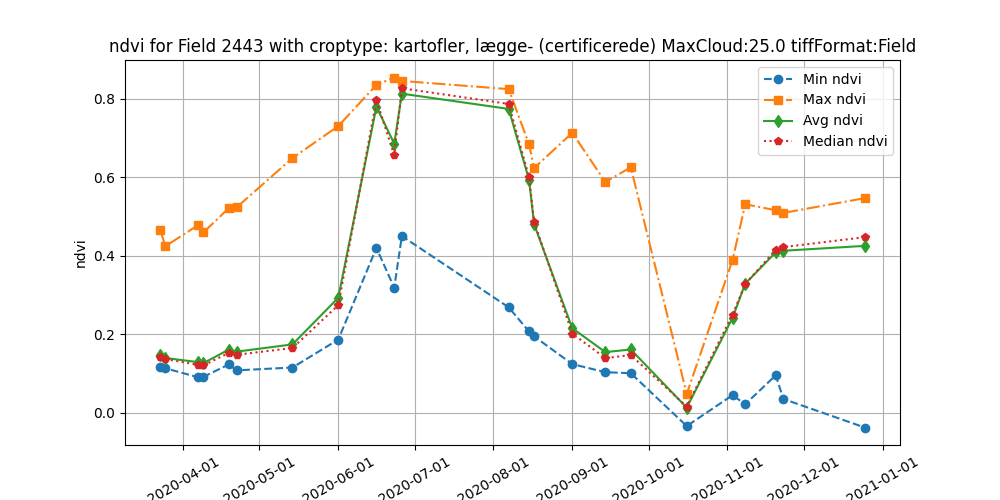
\includegraphics[width=0.75\linewidth]{images//results/Field2443NDVIGraph.png}
    \caption{NDVI readings for Field ID 2443, seed potatoes (25\% max cloud coverage)}
    \label{fig:2443NDVIavg}
\end{figure}

As a preliminary, there are data points missing. Even though the Sentinel-2 satellites circle Denmark every 3-5 day, if the cloud cover is significant enough there is too much noise to give accurate readings for vegetation indices. Because of this, any day with available data where the cloud coverage was over 25\% is excluded.

Aforementioned in the domain analysis, seed potatoes are planted late March throughout April. During the period the field should be rather barren and NDVI values low, in accordance to the figure. The max NDVI readings are higher. Assumably because of stray weeds or perhaps the polygon geometry had some inaccuracies and  included some flora, bushes or trees. Assuming the potatoes were planted mid to late April, the NDVI readings start increasing in the middle of May in accordance to the 2-6 weeks germination period. Throughout June and July an average NDVI reading of just below 0,8 is observed, indicating healthy dense vegetation. This is should be the case, as the canopy of the potato plants has a dense leaf area coverage.

On August 7th the average NDVI value is still saturated just below 0,8. But on the next reading on August 15th, the readings have dropped to just below 0,6. Such a significant drop provokes the assumption of pre-harvest crop desiccant usage. This drop in NDVI value continues throughout August and levels out in the middle to late September. This 20 day significant drop in NDVI value is in accordance with the desiccation time of desiccant Mizuki, as described in section \ref{Pre-harvest desiccation agents}. An assumption can be made on the basis of popularity and desiccation time, that Mizuki was used on or shortly after August 10th.

During this period it is observed that the maximum NDVI value fluctuates a bit and does not have a drop off like the average NDVI. This could be the result of stray weeds taking advantage of newly available sunlight, as the potato canopies wilt. But on the 16th October it drops to near 0 along with the average. It is assumed that harvest happened on or around the 16th, turning over all of the plants, leaving only soil visible. The next available reading is on the 29th of October and the NDVI value increases again, presumably due to weeds and other natural flora beginning to grow on the empty field.

\subsubsection{Heat maps}
These assumptions can be further explored using heat maps during the period of interest, August throughout October. The full set of heat maps over the period can be seen in appendix \ref{EvaluationResults}. 

\begin{figure}[htbp]
  \centering
  \begin{minipage}[b]{0.40\textwidth}
    \centering
    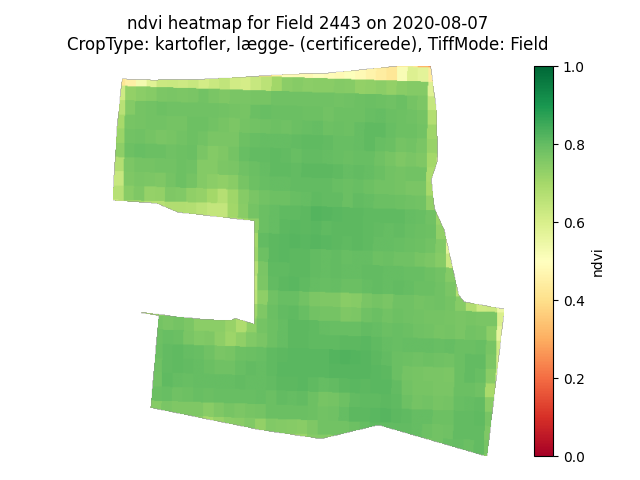
\includegraphics[width=\textwidth]{images/results/HeatmapsNDVI2443/HeatMapndvi_2443_kartofler_lgge-_certificerede_2020-08-07_Field.png}
    \caption{NDVI Heatmap August 7th (25\% max cloud coverage)}
    \label{fig:Heatmap7thAugust}
  \end{minipage}
  \hfill
  \begin{minipage}[b]{0.40\textwidth}
    \centering
    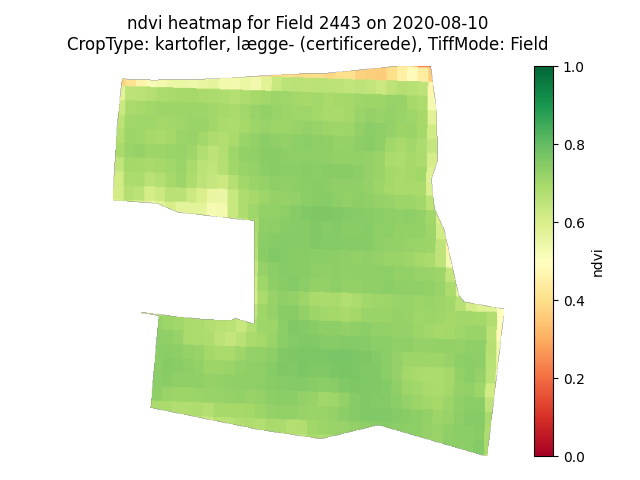
\includegraphics[width=\textwidth]{images/results/HeatmapsNDVI2443/HeatMapndvi_2443_kartofler_lgge-_certificerede_2020-08-10_Field.png}
    \caption{NDVI Heatmap August 10th (25\% max cloud coverage)}
    \label{fig:Heatmap10thAugust}
  \end{minipage}
\end{figure}
The assumed indication of pre-harvest crop desiccant use on August 7th. On figure \ref{fig:Heatmap7thAugust} the field is green and rather saturated. Notably, in the top right of the figure the values are rather low at approximately 0,5. It is assumed that there was not space for another trench to plant potatoes there and that section of the field did not contain any potato plants. Three days later an approximate 0.1 drop in NDVI value can be seen across the field, as seen on figure \ref{fig:Heatmap10thAugust}. On August 15th \ref{fig:Heatmap15thAugust} the average NDVI value is around 0,6. Such a drop in NDVI values is a clear indicator of stressed vegetation. And since it is in the pre-harvest crop desiccation usage period, it is further assumed to be the causation.

\begin{figure}[htbp]
  \centering
  \begin{minipage}[b]{0.40\textwidth}
    \centering
    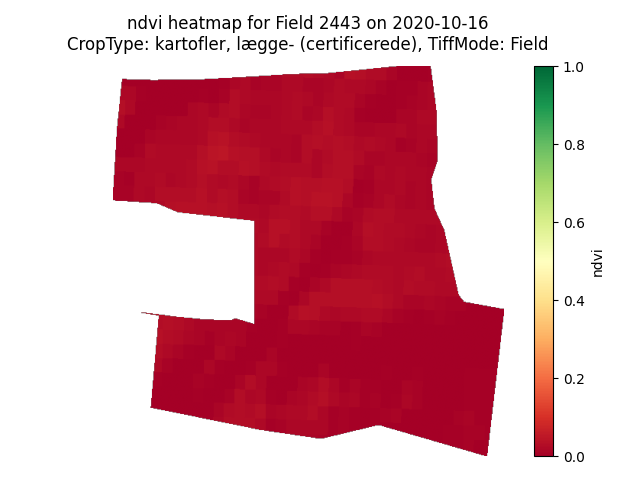
\includegraphics[width=\textwidth]{images/results/HeatmapsNDVI2443/HeatMapndvi_2443_kartofler_lgge-_certificerede_2020-10-16_Field.png}
    \caption{NDVI Heatmap October 16th (25\% max cloud coverage)}
    \label{fig:Heatmap16thOctober}
  \end{minipage}
  \hfill
  \begin{minipage}[b]{0.40\textwidth}
    \centering
    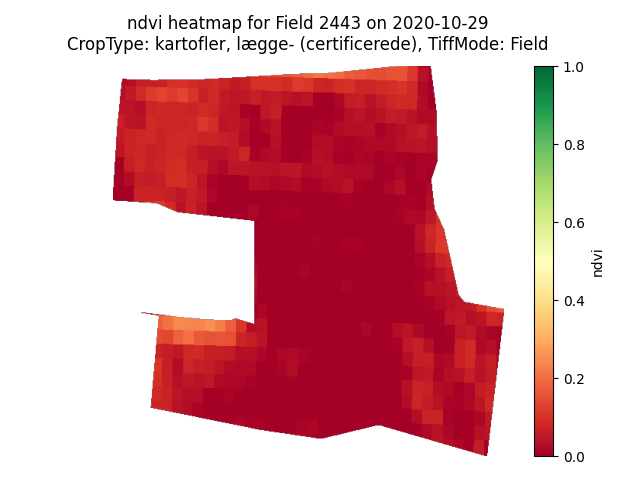
\includegraphics[width=\textwidth]{images/results/HeatmapsNDVI2443/HeatMapndvi_2443_kartofler_lgge-_certificerede_2020-10-29_Field.png}
    \caption{NDVI Heatmap October 29th (25\% max cloud coverage)}
    \label{fig:Heatmap29thOctober}
  \end{minipage}
\end{figure}

It is further solidified that the harvest came on or around October 16th when looking at figure \ref{fig:Heatmap29thOctober}, as the entire field is dark red signifying no vegetative growth on the field. Notably, the top right of the field is also dark red. This indicates that it was not bushes or trees overlapping on the field. Why the NDVI readings in that section were lower on the previous readings (figure \ref{fig:Heatmap7thAugust} and \ref{fig:Heatmap10thAugust}) is unknown. Perhaps potatoes were not planted there due to lack of space in terms of trench spacing. Or maybe that segment of the field was not properly fertilized and the potatoes growing there lacked the proper nutrients, leading to lower chlorophyll levels and in turn, NDVI levels. In correlation with figure \ref{fig:2443NDVIavg}, figure \ref{fig:Heatmap29thOctober} shows minor vegetation starting to sprout after the harvest around October 16th on the next available reading, the October 29th.

\subsection{Other vegetation indices}
In the domain analysis in section \ref{Vegetation indices}, a series of different vegetation indices were analysed, in regards to their ranges, spectral bands and specific use cases they are best suited for. This section analyses the results of other vegetation indices and explores whether they are better suited or can compliment the NDVI index, in the pursuit of detecting pre-harvest crop desiccant overuse.

While CVI is focused on detecting stressed vegetation, it is most commonly used to detect nutrient deficiencies in the soil, which in turn leads to stressed vegetation, in the early to mid growth period. Additionally, it does not have a normalized range and is context based, making it difficult to compare directly with NDVI.

Both EVI and GNDVI show the same story of the growth period of the potatoes as NDVI as seen on figure \ref{fig:2443GNDVIavg} and \ref{fig:2443EVIavg} (\ref{fig:Append2443GNDVIavg} \& \ref{fig:Append2443GNDVIavg} for larger pictures), but with some variance. \textcolor{red}{Anton vi skal lige have tjekket vores EVI formula, grafen er over 1, hvilket ikke burde være muligt. Men forventer dens værdier burde være lidt under NDVI, hvis den bliver beregnet korrekt?}

\begin{figure}[htbp]
  \centering
  \begin{minipage}[b]{0.42\textwidth}
    \centering
    \includegraphics[width=\textwidth]{images/results/Field2443GNDVIGraph.png}
    \caption{GNDVI readings for Field ID 2443, seed potatoes (25\% max cloud coverage)}
    \label{fig:2443GNDVIavg}
  \end{minipage}
  \hfill
  \begin{minipage}[b]{0.42\textwidth}
    \centering
    \includegraphics[width=\textwidth]{images/results/Field2443EVIGraph.png}
    \caption{EVI readings for Field ID 2443, seed potatoes (25\% max cloud coverage)}
    \label{fig:2443EVIavg}
  \end{minipage}
\end{figure}

EVI specializes in variability of crop development in relation to the leaf area index - bla bla ikke relevant index, videre
\textcolor{red}{EVI snak her - Skal have dobbelttjekket graf inden tho}

GNDVI does not saturate the same way NDVI does and generally has slightly lower values. But due to the green band focusing on green light reflectance off of chlorophyll, it is better at observing variance in chlorophyll levels across a vegetated area. \textcolor{red}{Mangler heatmaps her, har en teori om at der er større variance fra pixel til pixel med GNDVI? Krydser fingre}.

While GNDVI is more sensitive to variance in chlorophyll levels in plants and is most commonly used to detect stressed or aged vegetation in the intermediate to late growth stages. But similar to NDVI, its readings stem primarily from the canopy of the plant and the chlorophyll levels of the leaves, making it too similar in its usage.

\subsection{NDVI and NDRE readings}
Normalized Difference Red Edge Index is akin to GNDVI. It focuses of the chlorophyll levels of crops in the mid to late season, but differentiates itself by using the red edge spectrum, allowing it to "see" through the canopy, getting a fuller picture of the plants health. This has relevancy in multiple scenarios. Firstly, in the late season, if a crop is unaffected by pre-harvest crop desiccants and allowed its natural conclusion, the canopy will start to wilt. This will result in the NDVI values dropping, indicating stressed vegetation, which could be cause of alarm. But looking at an NDRE reading of the same crop, the readings might remain less affected as the vegetation beneath the canopy is still healthy\cite{eos_ndre}. In contrast, if the tuber or the stem of a crop becomes sick or lacks the proper nutrients, the canopy might still appear healthy. Here the NDVI values would remain high but a drop would be seen in the NDRE readings\cite{eos_ndre}.

Using NDVI and NDRE in combination is useful in determining the overall health of a crop, but it could also prove useful in determining the overuse of pre-harvest crop desiccants.

\begin{figure}[htbp]
    \centering
    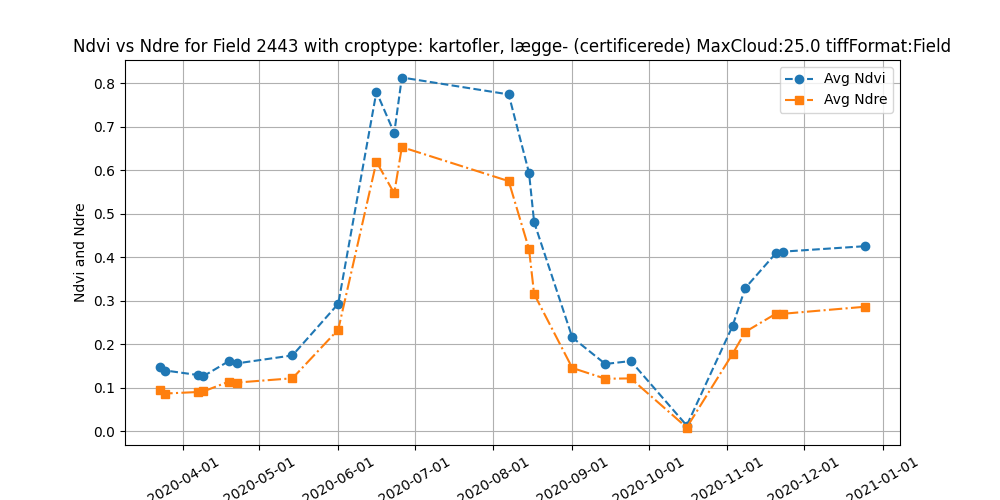
\includegraphics[width=0.75\linewidth]{images//results/Field2443NDREandNDVI.png}
    \caption{NDVI \& NDRE readings for Field ID 2443, seed potatoes (25\% max cloud coverage)}
    \label{fig:2443NDVIandNDREavg}
\end{figure}

Inspecting the same field using NDVI and NDRE on figure \ref{fig:2443NDVIandNDREavg}, it is expected to see NDRE follow along with NDVI throughout the growth cycle of the potato plant. It has a lower value than NDVI, which is expected, as the NDRE does not saturate like NDVI does and pierces to canopy to gets a clearer reading of the overall chlorophyll levels. Around August 7th where assumed pre-harvest crop desiccant application occurs, both indices drop significantly. Notably, the NDVI has a steeper decline over the desiccation period than the NDRE index. This could be because the crop desiccant is sprayed in liquid form and while it should kill both the leaves and the stem, it primarily hits the leaves, leading to a quicker wilting of the canopy and in turn steeper drop in NDVI values compared to NDRE values. This could also be why multiple applications of crop desiccants can be necessary. \textcolor{red}{Sidste assumption her skal jeg lige se om jeg kan undersøge og finde en kilde på}
Notably, both indices plateau at around 0,1 NDRE and 0,15 NDIin the middle of September, indicating the vegetation is dead and wilted. And both indices reach a value of near 0 on at harvest around October 16th.

\subsubsection{Heat maps}
\textcolor{red}{Faktisk lidt usikker på hvad jeg vil sige med heatmaps her? Måske bare lidt sådan "uha se der er varians", men idk. Virker lidt luftigt}

\subsection{Theoretical Pesticide Overuse Calculations} \label{Theoretical Pesticide Overuse Calculations}
Observed on figure \ref{fig:2443NDVIandNDREavg} the NDVI has a steeper decline compared to the NDRE index on August 7th, the assumed date of pre-harvest crop desiccant application. It is theorized that the causation for this is because the desiccant primarily hits the leaves, leading to a quicker wilting of the canopy and a faster decline in the NDVI. But should an overuse of pesticides be used, it is assumed that there would be a more thorough application to the entirety of the plant, including the stem, illustrated on figure \ref{fig:overuseIllustration}, which would lead to a steeper decline of the NDRE index.

\begin{figure}[htbp]
    \centering
    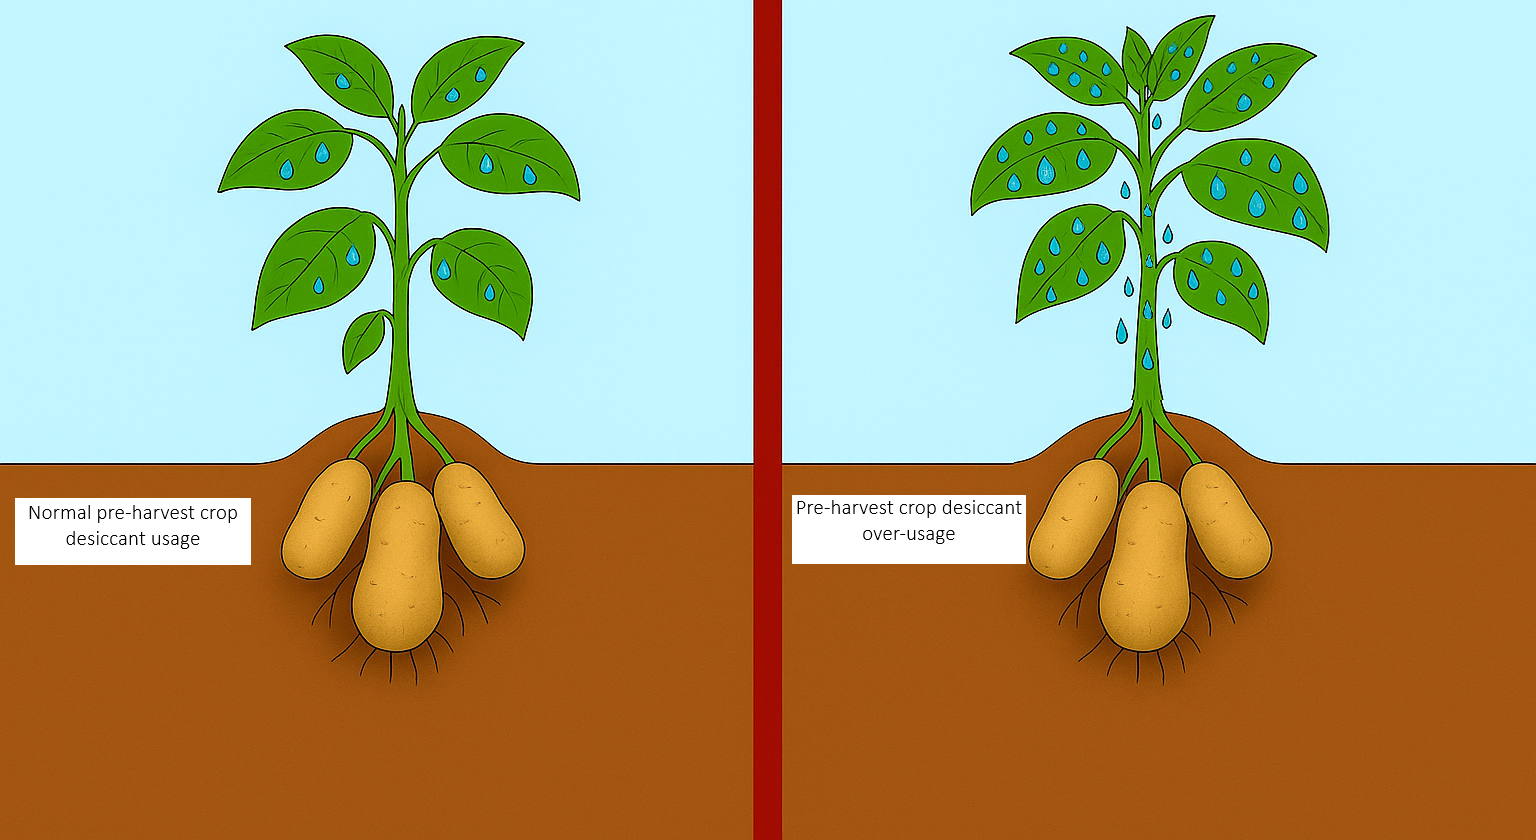
\includegraphics[width=0.75\linewidth]{images//results/potatovaffleri2.png}
    \caption{Theoretical Pre-harvest Desiccant Application and Overuse Application (generated from sketch using AI)}
    \label{fig:overuseIllustration}
\end{figure}

The following is a theoretical approach of finding trends that could be an indication of pre-harvest crop desiccant overuse. The approach is based of of NDVI being predominantly sensitive to leaf canopy degradation, while NDRE can penetrate deeper to asses overall biomass health and stress and how an overuse of desiccant agents would assumably affect the entirety of the plant more thoroughly, leading to a quicker decline of stem health along with the canopy.

On figure \ref{fig:Field2443Geogebra} the diagram has been plotted in GeoGebra and two linear lines have been drawn for NDVI and NDRE respectively. The pre crop desiccant use line (pre-line), is the best fitted linear line going through all of the points from the healthiest stage in June (highest chlorophyll levels) till the last point before the decline indicating crop desiccant use. And the post crop desiccant use line (post-line), which is the best fitted linear line going through all of the points from the start of the decline till the plateau.

\begin{figure}[htbp]
    \centering
    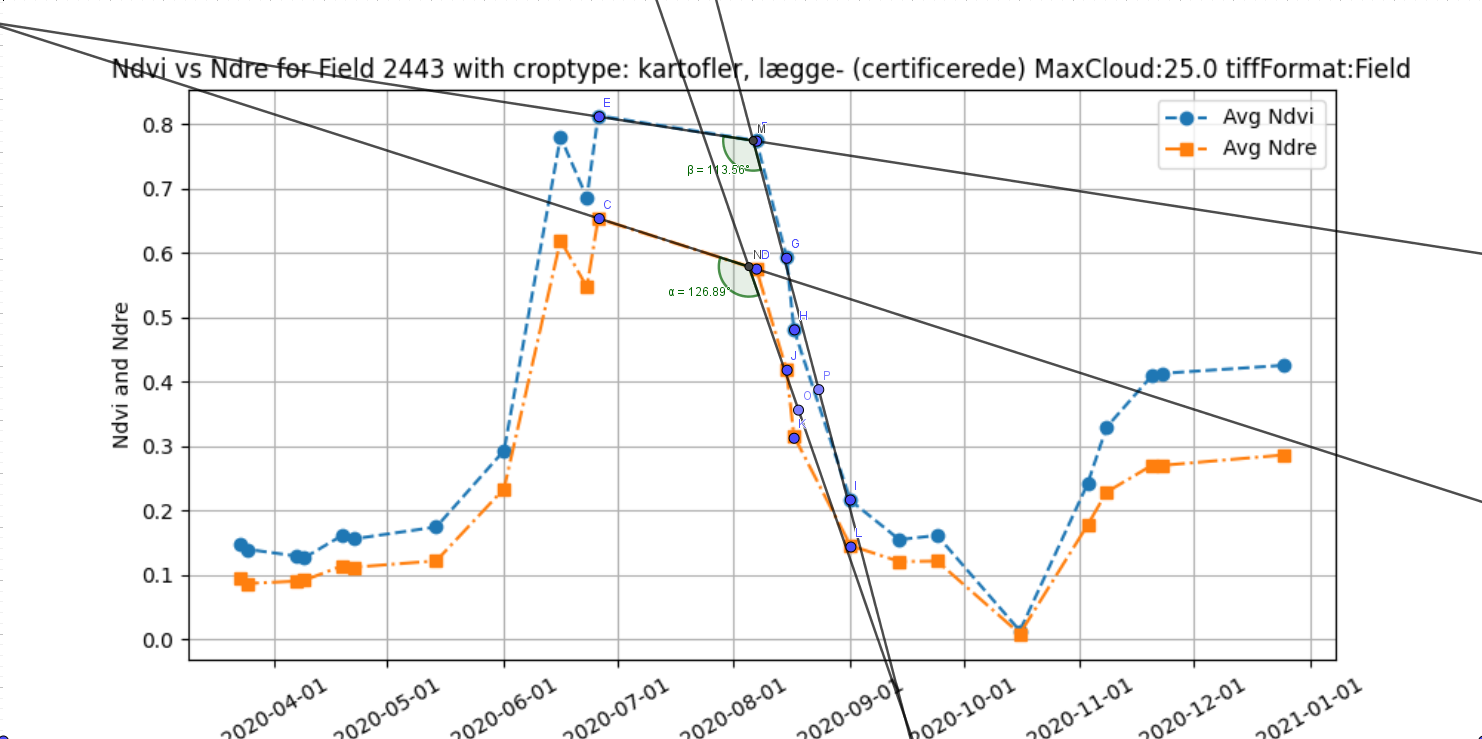
\includegraphics[width=0.75\linewidth]{images//results/Field2443Geogebra.png}
    \caption{Field 2443 angle analysis between pre- and post desiccant application linear decline}
    \label{fig:Field2443Geogebra}
\end{figure}

Measuring the angle between the pre-line and post-line for NDVI and NDRE, the NDRE angle should generally be broader compared to the NDVI angle, as the the NDVI post-line has a steeper decline. Comparing the two can be done by simple division of the two:

\begin{equation}
    \text{Overuse Score} = \frac{\text{NDVI-Angle}}{\text{NDRE-Angle}}
    \label{eq:overuse_score}
\end{equation}

This was done with a number of different fields growing seed potatoes in Denmark in the same year, where the graphs were plotted and the overuse score was calculated, as seen on table \ref{tab:field_overuse_scores}.

\begin{table}[htbp]
    \centering
    \begin{tabular}{cc}
        \hline
        \textbf{Field ID} & \textbf{Overuse Score} \\
        \hline
        2443 & 0,895 \\
        6079 & 0,887 \\
        8744 & 0,896 \\
        9530 & 1,07 \\
        9661 & 0,99 \\
        \hline
    \end{tabular}
    \caption{Field ID and Corresponding Overuse Scores}
    \label{tab:field_overuse_scores}
\end{table}

Using this logic, a clear trend emerges. The normal overuse scores lie around 0,9 and the closer they are to 1 or greater than 1, the greater the likelihood of desiccant overuse. An issue with this method is the lack of data due to cloud coverage. If the cloud coverage is greater than 25\% that days data point was excluded because of the extremity is noise levels. This presents the problem that some fields experienced long periods of cloudy days and lack data points. An example of this is seen on figure \ref{fig:Field9530Geogebra}

\begin{figure}[htbp]
    \centering
    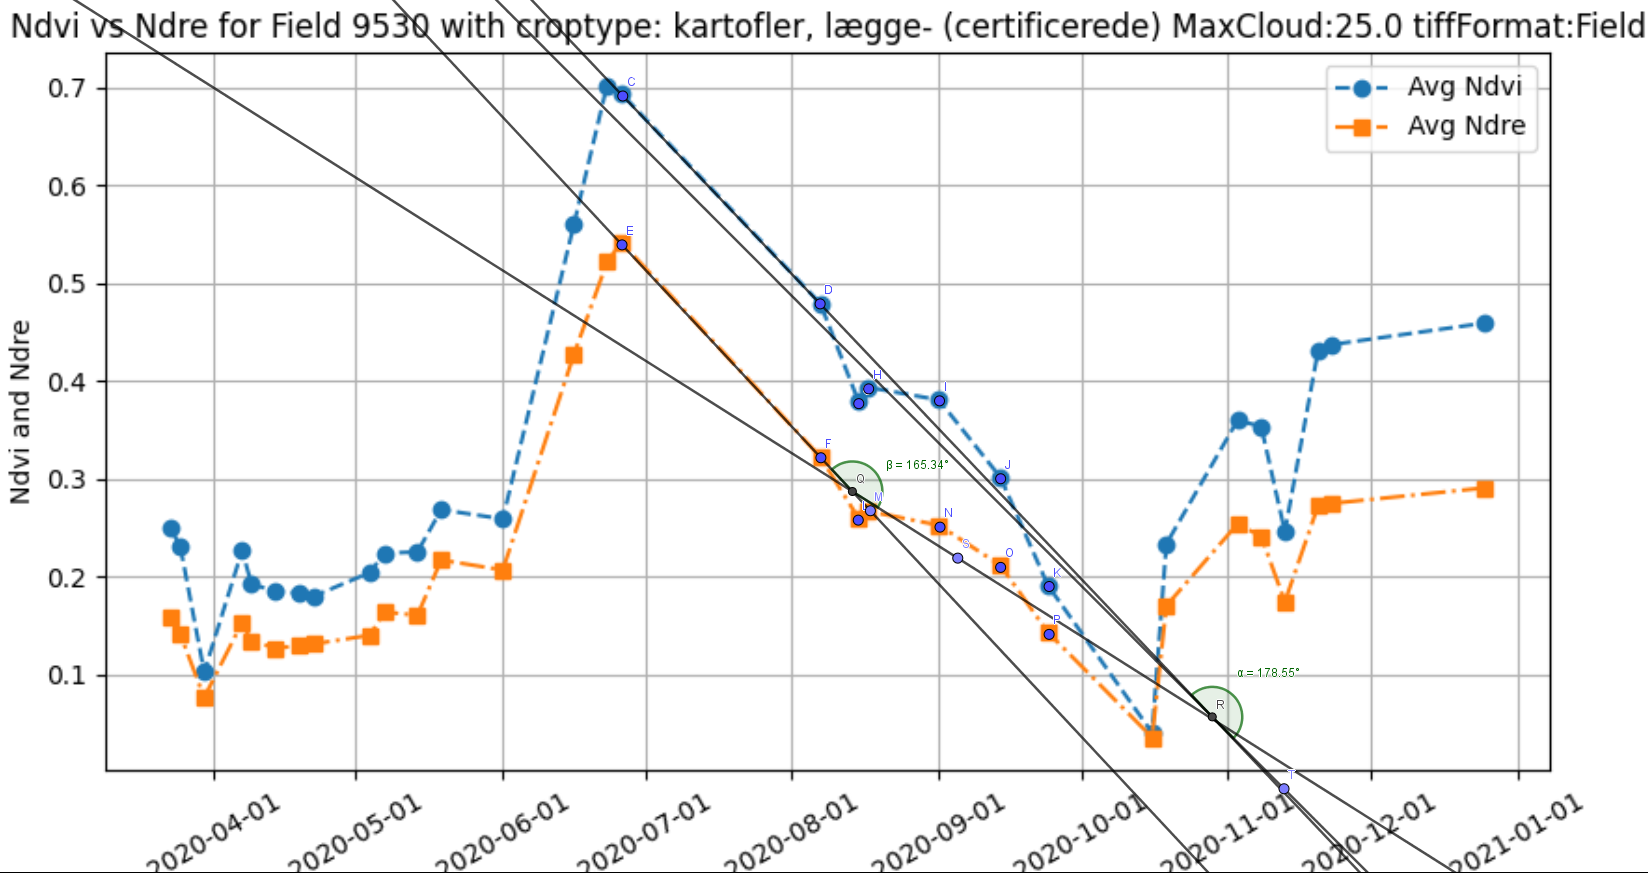
\includegraphics[width=0.75\linewidth]{images//results/Field9530Geogebra.png}
    \caption{Field 9530 angle analysis between pre- and post desiccant application linear decline}
    \label{fig:Field9530Geogebra}
\end{figure}
\chapter{Discussion} \label{Discussion}
\chapter{Future Work} \label{Future Work}
\chapter{Conclusion} \label{Conclusion}
\newpage

\appendix

\chapter{Source code} \label{SourceCode}

The source code for the plug-in is available at this URL: \url{https://github.com/...}.

The source code for the underlying ...: \url{https://github.com/...}.
\chapter{Requirements}
The full functional requirements table can be seen in \ref{Ap_LongReqTable}

\begin{longtable}{|p{1.2cm}|p{4cm}|p{6cm}|p{1.2cm}|}
\caption{Full Functional Requirements table with MoSCoW prioritization \label{Ap_LongReqTable}}\\

\hline
\textbf{ID} & \textbf{Name} & \textbf{Description} & \textbf{Voting} 
\endfirsthead


\multicolumn{4}{c}{Continuation of Table \ref{Ap_LongReqTable}} \\
\hline
\textbf{ID} & \textbf{Name} & \textbf{Description} & \textbf{Voting} 
\endhead

\hline
\multicolumn{4}{|r|}{\textit{Continued on next page}} \\
\hline
\endfoot

\hline
\endlastfoot

\hline
FR1 & Use the DEPA shapefiles & Read and unpack the shapefile dataset &\textbf{M}\\
\hline
FR1.1 & Extract Fields & Extract fields with the correct crop type & \textbf{M} \\
\hline
FR1.1.1 & User-defined crop type & Allow user to select a given crop type to extract & \textbf{C} \\
\hline
FR1.1.2 & Insert into DB & Store extracted fields in a database for NDVI association & \textbf{M} \\
\hline
FR2 & Download remote sensing data & Handle download of remote sensing data from the Sentinel-2 satellites & \textbf{M}\\
\hline
FR2.1 & Identify available dates & Find dates for a given field with available sensing data & \textbf{S} \\
\hline
FR2.2 & API Authentication & Authenticate to Sentinel APIs before making calls & \textbf{M} \\
\hline
FR2.3 & Download images & Download satellite images with required bands for specific dates & \textbf{M} \\
\hline
FR2.3.1 & Flexible download area & Allow user to select between large Denmark section or specific fields & \textbf{C} \\
\hline
FR2.3.2 & Download options & Provide download options for list of fields and resolution &\textbf{C} \\
\hline
FR3 & Process Satellite images & Handle image analysis workflows &\textbf{M} \\
\hline
FR3.1 & Calculate NDVI & Calculate NDVI per pixel from image data &\textbf{M} \\
\hline
FR3.2 & Validate pixel data & Ensure there is valid data before calculating NDVI &\textbf{M} \\
\hline
FR3.3 & Overuse score & Use NDVI to infer possible pesticide overuse & \textbf{M} \\
\hline
FR3.3.1 & Ai & Train Ai on NDVI Data to infor Possible pesticide overuse & \textbf{W}\\
\hline
FR3.3.2 & Statistical model & Calculate possible pesticide overuse based on a Statistical model & \textbf{M} \\
\hline
FR3.4 & Other indices & Calculate additional green indices for better insights & \textbf{C} \\
\hline
FR3.5 & Store Data & Store the calculated data to use in future & \textbf{S} \\
\hline
FR4 & Show results & Display outputs through a GUI or reports & \textbf{S} \\
\hline
FR4.1 & Color-coded map & Map of Denmark with color-coded potato fields indicating risk level & \textbf{W} \\
\hline
FR4.2 & List of fields & List of fields likely to have overused pesticide & \textbf{S} \\
\hline
FR4.3 & Data exploration & (rewrite)Plot NDVI and other data over time & \textbf{C} \\
\hline
FR4.3.1 & Make image plots & (rewrite)Make the images into Heatmaps to locate hot spots & \textbf{C} \\
\hline
FR5 & Delegate work & Implement a work queue for long tasks like downloading and processing & \textbf{M} \\
\hline
FR6 & Integration & Integrate with DEPA's system & \textbf{C} \\
\hline
FR7 & Error Handling & Log and report API or processing errors clearly & \textbf{S} \\
\hline
FR8 & Data Export & Allow exporting results as CSV, GeoJSON, or PDF & \textbf{C} \\
\hline
FR9 & Notifications & Notify user when processing or downloading completes & \textbf{W} \\
\hline
\end{longtable}
\chapter{Evaluation Results} \label{EvaluationResults}

\section{Field 2443 Heatmaps}

\begin{figure}[htbp]
  \centering
  \begin{minipage}[b]{0.40\textwidth}
    \centering
    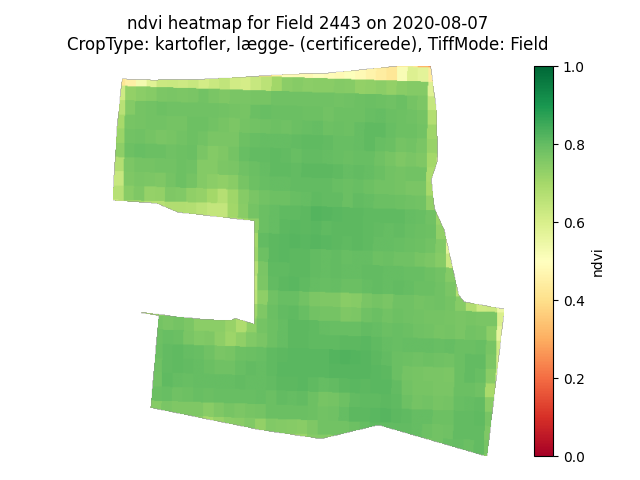
\includegraphics[width=\textwidth]{images/results/HeatmapsNDVI2443/HeatMapndvi_2443_kartofler_lgge-_certificerede_2020-08-07_Field.png}
    \caption{NDVI Heatmap August 7th (25\% max cloud coverage)}
    \label{fig:AppHeatmap7thAugust}
  \end{minipage}
  \hfill
  \begin{minipage}[b]{0.40\textwidth}
    \centering
    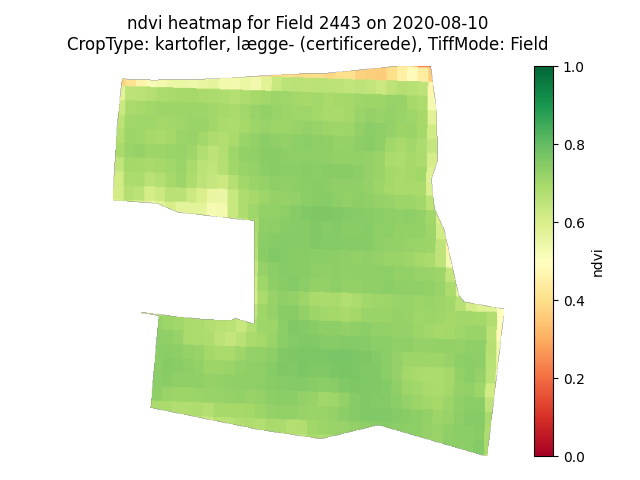
\includegraphics[width=\textwidth]{images/results/HeatmapsNDVI2443/HeatMapndvi_2443_kartofler_lgge-_certificerede_2020-08-10_Field.png}
    \caption{NDVI Heatmap August 10th (25\% max cloud coverage)}
    \label{fig:AppHeatmap10thAugust}
  \end{minipage}
\end{figure}

\begin{figure}[htbp]
  \centering
  \begin{minipage}[b]{0.40\textwidth}
    \centering
    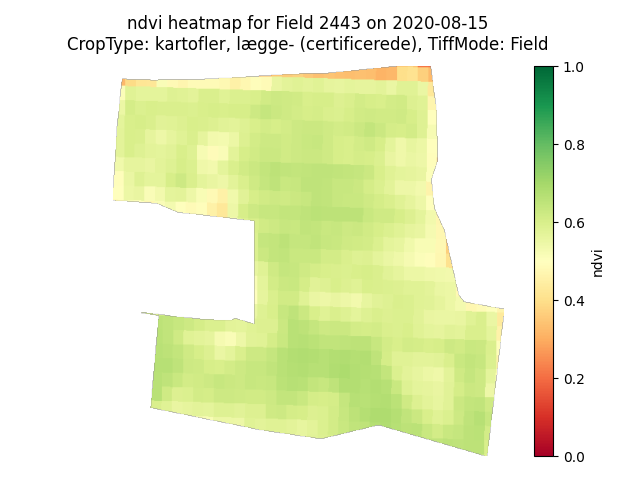
\includegraphics[width=\textwidth]{images/results/HeatmapsNDVI2443/HeatMapndvi_2443_kartofler_lgge-_certificerede_2020-08-15_Field.png}
    \caption{NDVI Heatmap August 15th (25\% max cloud coverage)}
    \label{fig:Heatmap15thAugust}
  \end{minipage}
  \hfill
  \begin{minipage}[b]{0.40\textwidth}
    \centering
    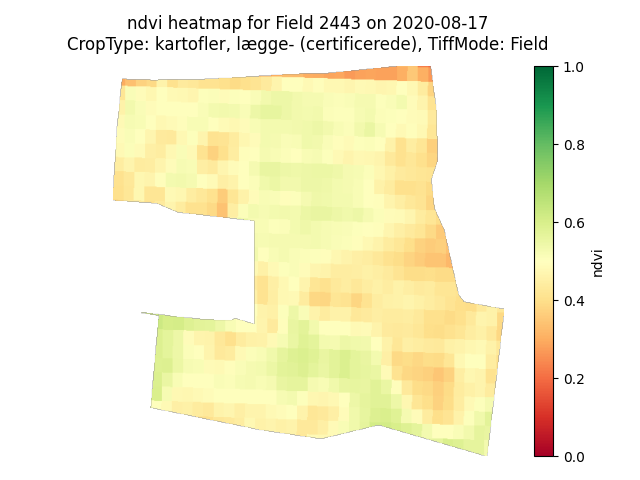
\includegraphics[width=\textwidth]{images/results/HeatmapsNDVI2443/HeatMapndvi_2443_kartofler_lgge-_certificerede_2020-08-17_Field.png}
    \caption{NDVI Heatmap August 17th (25\% max cloud coverage)}
    \label{fig:Heatmap17thAugust}
  \end{minipage}
\end{figure}

\begin{figure}[htbp]
  \centering
  \begin{minipage}[b]{0.40\textwidth}
    \centering
    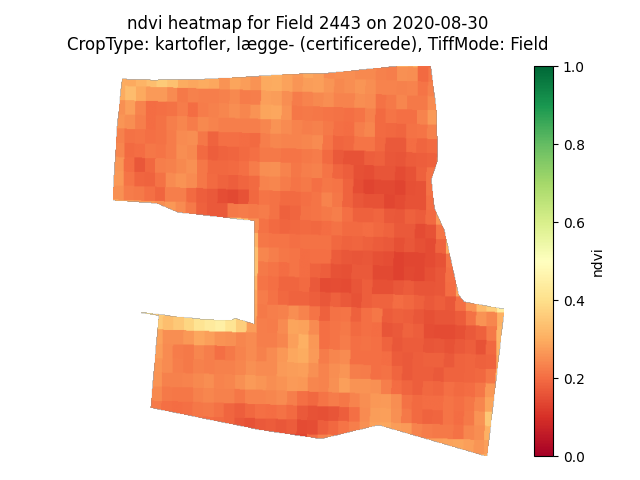
\includegraphics[width=\textwidth]{images/results/HeatmapsNDVI2443/HeatMapndvi_2443_kartofler_lgge-_certificerede_2020-08-30_Field.png}
    \caption{NDVI Heatmap August 30th (25\% max cloud coverage)}
    \label{fig:Heatmap30thAugust}
  \end{minipage}
  \hfill
  \begin{minipage}[b]{0.40\textwidth}
    \centering
    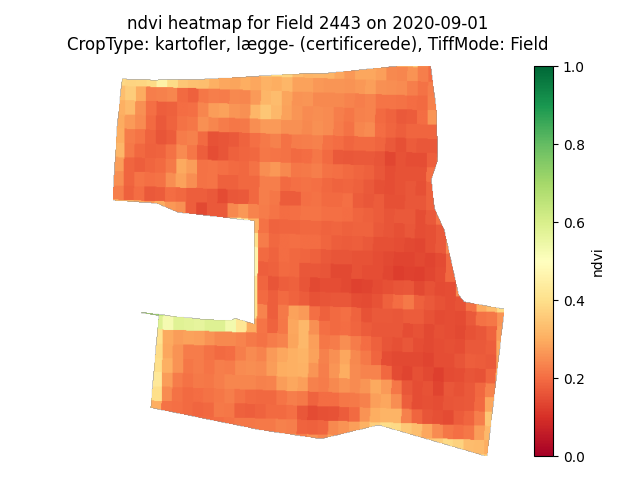
\includegraphics[width=\textwidth]{images/results/HeatmapsNDVI2443/HeatMapndvi_2443_kartofler_lgge-_certificerede_2020-09-01_Field.png}
    \caption{NDVI Heatmap September 1st (25\% max cloud coverage)}
    \label{fig:Heatmap1stSeptember}
  \end{minipage}
\end{figure}

\begin{figure}[htbp]
  \centering
  \begin{minipage}[b]{0.40\textwidth}
    \centering
    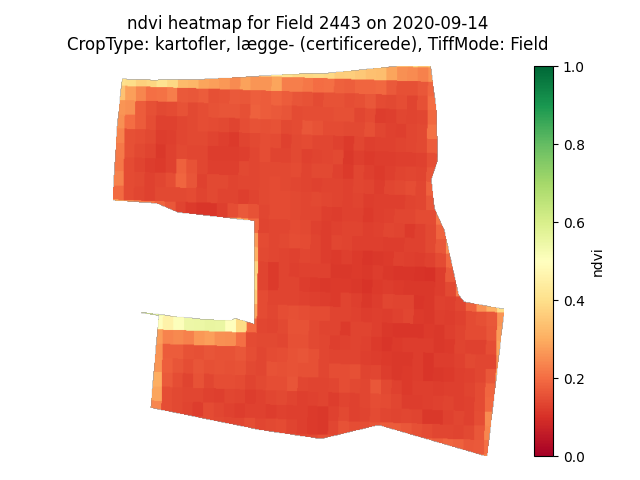
\includegraphics[width=\textwidth]{images/results/HeatmapsNDVI2443/HeatMapndvi_2443_kartofler_lgge-_certificerede_2020-09-14_Field.png}
    \caption{NDVI Heatmap September 14th (25\% max cloud coverage)}
    \label{fig:Heatmap14thSeptember}
  \end{minipage}
  \hfill
  \begin{minipage}[b]{0.40\textwidth}
    \centering
    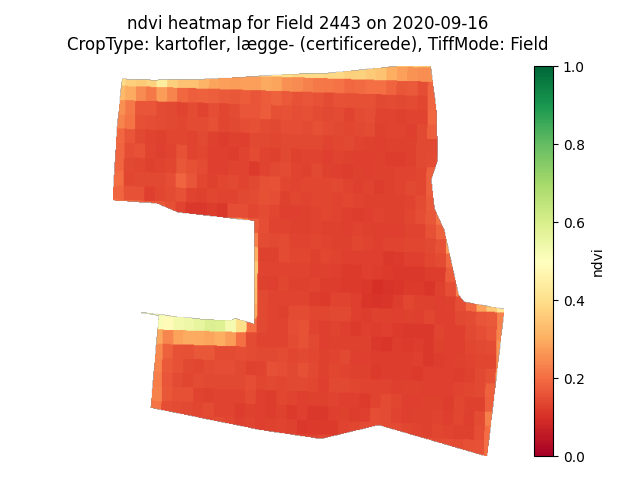
\includegraphics[width=\textwidth]{images/results/HeatmapsNDVI2443/HeatMapndvi_2443_kartofler_lgge-_certificerede_2020-09-16_Field.png}
    \caption{NDVI September August 16th (25\% max cloud coverage)}
    \label{fig:Heatmap16thSeptember}
  \end{minipage}
\end{figure}

\begin{figure}[htbp]
  \centering
  \begin{minipage}[b]{0.40\textwidth}
    \centering
    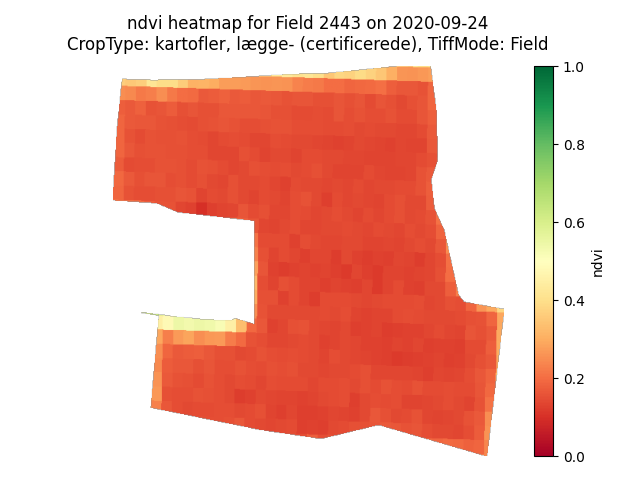
\includegraphics[width=\textwidth]{images/results/HeatmapsNDVI2443/HeatMapndvi_2443_kartofler_lgge-_certificerede_2020-09-24_Field.png}
    \caption{NDVI Heatmap September 24th (25\% max cloud coverage)}
    \label{fig:Heatmap24thSeptember}
  \end{minipage}
  \hfill
  \begin{minipage}[b]{0.40\textwidth}
    \centering
    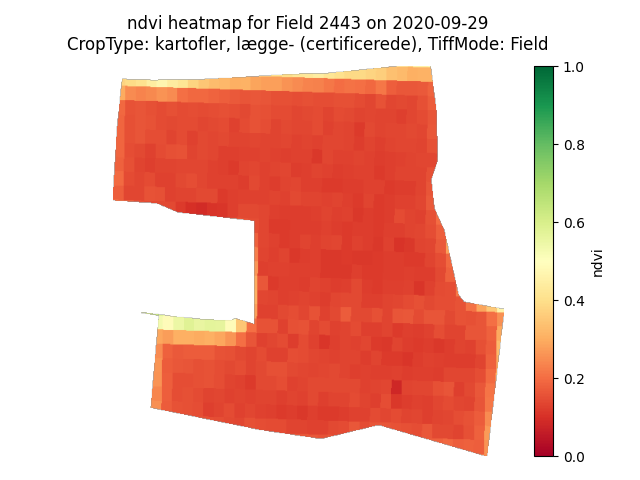
\includegraphics[width=\textwidth]{images/results/HeatmapsNDVI2443/HeatMapndvi_2443_kartofler_lgge-_certificerede_2020-09-29_Field.png}
    \caption{NDVI Heatmap September 29th (25\% max cloud coverage)}
    \label{fig:Heatmap29thSeptember}
  \end{minipage}
\end{figure}

\begin{figure}[htbp]
  \centering
  \begin{minipage}[b]{0.40\textwidth}
    \centering
    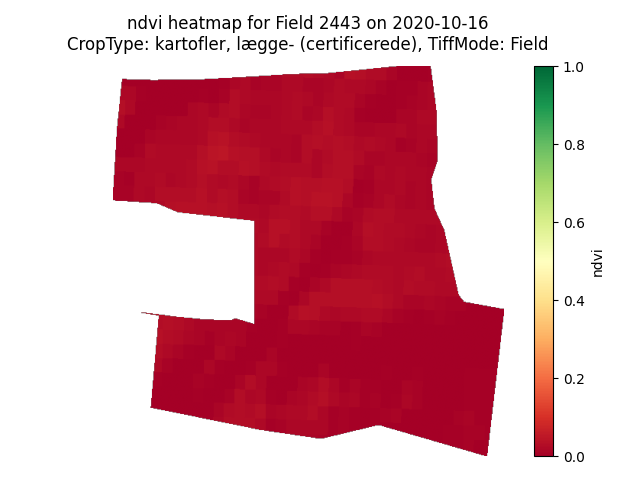
\includegraphics[width=\textwidth]{images/results/HeatmapsNDVI2443/HeatMapndvi_2443_kartofler_lgge-_certificerede_2020-10-16_Field.png}
    \caption{NDVI Heatmap October 16th (25\% max cloud coverage)}
    \label{fig:AppendHeatmap16thOctober}
  \end{minipage}
  \hfill
  \begin{minipage}[b]{0.40\textwidth}
    \centering
    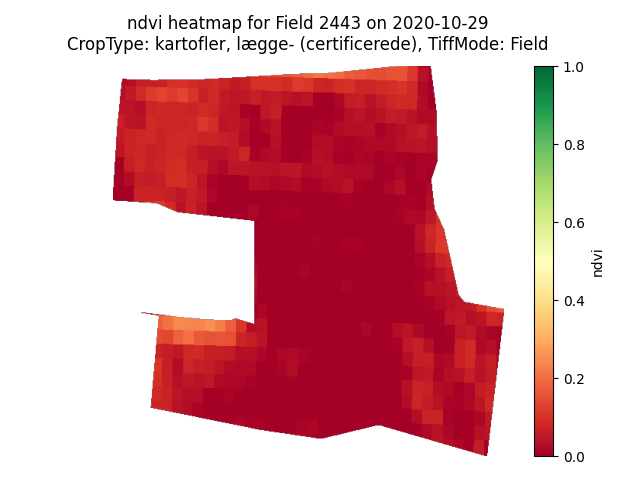
\includegraphics[width=\textwidth]{images/results/HeatmapsNDVI2443/HeatMapndvi_2443_kartofler_lgge-_certificerede_2020-10-29_Field.png}
    \caption{NDVI Heatmap October 29th (25\% max cloud coverage)}
    \label{fig:AppendHeatmap29thOctober}
  \end{minipage}
\end{figure}

\begin{figure}[h]
    \centering
    \includegraphics[width=0.75\linewidth]{images//results/Field2443GNDVIGraph.png}
    \caption{NDVI readings for Field ID 2443, seed potatoes (25\% max cloud coverage)}
    \label{fig:Append2443GNDVIavg}
\end{figure}

\begin{figure}[h]
    \centering
    \includegraphics[width=0.75\linewidth]{images//results/Field2443EVIGraph.png}
    \caption{NDVI readings for Field ID 2443, seed potatoes (25\% max cloud coverage)}
    \label{fig:Append2443EVIavg}
\end{figure}

%\bibliographystyle{splncs04}
%\bibliography{references}
\printbibliography

\end{document}